\chapter{Principal component analysis}
\label{pca}


The origins of principal component analysis are usually traced to \cite{Pearson:1901} who was concerned with the fitting planes in the analysis of covariance matrices by orthogonal least squares.   Much development of the technique is ascribed to \cite{Hotelling:1933}, who, working with the correlation matrix provided another development of the technique which is more familiar.    As a technique in its own right it has received book length treatment by \cite{Jackson:1991} and \cite{Jolliffe:1986}; another excellent exposition is given in \cite{Flury:1988} who also develops one generalisation of the technique to multiple groups.   The theory underlying principal components is important in a wide range of areas, consequently this chapter will examine some of the underlying theory as well as considering conventional approaches to principal component analysis.   An \textbf{R}-centric selection of recent extensions to the technique will also be considered in the next chapter.

Principal component analysis can be performed for a variety of reasons, one can perhaps consider its use in one of three ways.   Arguably the most common use is in terms of dimension reduction.   Principal component analysis can be thought of as a data analytic method which provides a specific set of projections\index{projections} which represent a given data set in fewer dimensions.   This has obvious advantages when it is possible to reduce dimensionality to two or three as visualisation becomes very straightforward but it should be acknowledged that reduced dimensionality has advantages beyond visualisation.  Another rationale for conducting principal components analysis is to transform correlated variables into uncorrelated ones, in other words to \emph{sphere} the data.   Whilst univariate data can be standardised by centering and scaling, in a multivariate context one may also wish to ``standardise'' the correlation between variables to zero.    The final rationale for the technique is that it finds linear combinations of data which have relatively large (or relatively small) variability.

In essence, we wish to form projections $\boldsymbol{z} = (z_{1}, z_{2}, \ldots, z_{q})$  of the \emph{standardised} data $\boldsymbol{x} = (x_{1}, x_{2}, \ldots, x_{p})$ 

\begin{eqnarray*}
z_{1} &=& e_{11} x_{1} + e_{12} x_{2} + \ldots e_{1p} x_{p}\\
z_{2} &=& e_{21} x_{1} + e_{22} x_{2} + \ldots e_{2p} x_{p}\\
\ldots\\
z_{q} &=& e_{q1} x_{1} + e_{q2} x_{2} + \ldots e_{qp} x_{p}
\end{eqnarray*}

where the coefficients  $\boldsymbol{E}$ form a $p \times q$ matrix.   If dimension reduction is our goal, clearly we hope that we can form an adequate representation of the data with $q<p$.   

We are going to illustrate Principal Component Analysis by reference to three sets of data.   The first was presented by \cite{Karlis+etal:2003} and relates to Heptathalon results from the Sydney Olympics in 2000.   In this event, athletes compete in seven different sporting activities, and clearly for the purposes of the competition a decision has to be made as to who is the best heptathelete overall.  For sporting purposes, points are awarded for performance in each event and summed.   In essence, a one dimensional composite variable has to be created from the results for the seven events before a decision can be made as to who wins the medals.   We are not necessarily going to challenge the way the International Olympic Committee calculates scores, but clearly a linear combination which achieved maximum separation of athletes might be interesting.   A trivial linear combination would be to take $\boldsymbol{e} = \frac{1}{n}\boldsymbol{1}$.   However, the aim of any projection method is to find an \emph{interesting} projection of the data.   All we need to do is decide what we mean by \emph{interesting}.   As mentioned earlier, one use of principal components is to find projections where the variance is maximised, thus maximising the separation between heptatheletes.  

The second rather well used set of data relates to carapace measurements the painted turtle \textit{Chrysemys picta marginata} first reported by \cite{Jolicoeur+Mosimann:1960}.   These data contain 3 variables recording the shell length, width and height for 24 male and 24 female turtles.   We will consider these data partly because the turtles are cute, but mainly because it affords some consideration of the role of standardisation.   Standardising by subtracting mean and dividing by the standard deviation can be a rather brutal approach, it is possible to take the natural logarithms of these anatomical measures which allows a different insight into the relationship between the measures.

Finally, we will investigate some gene expression data.   In microarray experiments, one typically collects data from a relatively small number of individuals, but records information on gene expression of a large number of genes and therefore have a data matrix $\boldsymbol{X}$ where $n << p$.   Dimension reduction is a central concern at some stage of the analysis, either on the whole set of genes or on a selected subset.   As might become clear, groups of genes which can be identified analytically as co-expressing are referred to as eigengenes.   We will therefore consider some of the issues surrounding the interpretation of principal components in high dimensions.

Some other data sets will be included to illustrate specific points where necessary, and the excercises will also develop other data sets.

%Signature components - linear combinations of the genes that belong to that ocmponent  The first pc is the best 1d representation of a signature component, if genes in a signature component are tightly expressed they will show high correlelation with the pc.  But orthogality, lack of correlation and indepence may be unnecessary requirements. - find loadings and rotate   Simple pca cannot be used with p >> n    -- but we don't want to explain max variance we really want max correlation.


\section{Derivation of Principal Components}

We will firstly consider the derivation of population principal components in the style proposed by \cite{Hotelling:1933} as a way of finding linear combinations with maximum variance.   Given that we have a random vector $\boldsymbol{x} \in \mathbb{R}^{P}$, we wish to consider the vector of transformed variables $\boldsymbol{z} = \boldsymbol{\alpha}^{T}(\boldsymbol{x} - \boldsymbol{\bar{x}})$, and so we wish to find $\alpha$ such that the $\mbox{Var}(z)$ is maximised.  By convention, we insist that $\boldsymbol{\alpha}$ is orthonormal, i.e. in addition to being a vector of unit length we require that $\boldsymbol{\alpha}^{T}\boldsymbol{\alpha} = 1$.   To find an expression for $\mbox{Var}(z)$ in terms of the original variables $\boldsymbol{x}$, firstly by considering the following relationship:
\begin{displaymath}
\mbox{Var}(\boldsymbol{z}) = \mbox{Var}(\boldsymbol{\alpha}^{T}\boldsymbol{x}) = E(\boldsymbol{\alpha}^{T}\boldsymbol{x})^{2}
\end{displaymath}
Hence,
\begin{displaymath}
\sum_{i+1}^{n}(\boldsymbol{z}_{i} - \boldsymbol{\bar{z}})^{2} = \sum_{i=1}^{n}\boldsymbol{\alpha}^{T}\left[(\boldsymbol{x}_{i} - \boldsymbol{\bar{x}})(\boldsymbol{x}_{i} - \boldsymbol{\bar{x}})^{T}\right] \boldsymbol{\alpha}
\end{displaymath}
and premultiplying both sides by $\frac{1}{n-1}$ gives us an estimate of the variance of the transformed variables in terms of the original variables.  To find $\boldsymbol{\alpha}$ in order to maximise the variance we therefore wish to find:  
\begin{equation}
\mbox{max}(\boldsymbol{\alpha}^{T}\boldsymbol{\hat{\Sigma}}\boldsymbol{\alpha})
\end{equation}
subject to the side condition that $\boldsymbol{\alpha}^{T}\boldsymbol{\alpha}= 1$.   Considering the first principal component, we wish to maximise $\mbox{Var}(z_{1}) = \boldsymbol{\alpha}_{1}^{T}\boldsymbol{\hat{\Sigma}}\boldsymbol{\alpha}_{1}$; it can be shown that this problem can be specified by incorporating a Lagrange multiplier.   Consider maximising the expression $\varphi$ given below, where $\lambda$ is a Lagrange multiplier:
\begin{equation}
\varphi_{1} = \boldsymbol{\alpha}_{1}^{T}\boldsymbol{\hat{\Sigma}}\boldsymbol{\alpha}_{1} - \lambda_{1}(\boldsymbol{\alpha}_{1}^{T}\boldsymbol{\alpha}_{1} - 1)
\end{equation}
which can be solved by differentiation with respect to $\boldsymbol{\alpha}_{1}$.   The differential gives us a system of linear equations as follows:
\begin{equation}
\frac{\partial \varphi_{1}}{\partial \boldsymbol{\alpha}_{1}} = 2 \Sigma \boldsymbol{\alpha}_{1} - 2 \lambda \boldsymbol{\alpha}_{1}
\end{equation}
and setting the derivative equal to zero gives:
\begin{equation}
\boldsymbol{\Sigma} \boldsymbol{\alpha}_{1} = \lambda_{1} \boldsymbol{\alpha}_{1}
\end{equation}
which is easily rearranged to give:
\begin{equation}
(\boldsymbol{\Sigma} - \lambda_{1} \boldsymbol{I})\boldsymbol{\alpha} = 0.
\end{equation}

We have $p$ equations and $p$ unknowns, but we can find non-trivial solutions where $\boldsymbol{\alpha} \neq \boldsymbol{0}$ noting that if  $\boldsymbol{a}_{1}^{T}\boldsymbol{a}= 1$ then $\boldsymbol{\Sigma} - \lambda \boldsymbol{I}$ is singular which therefore implies that:
\begin{equation}
|\boldsymbol{\Sigma} - \lambda_{1} \boldsymbol{I}| = 0
\end{equation}

This looks like an eigenproblem, so $\lambda_{1}$ can be found as the largest eigenvalue of $\boldsymbol{\Sigma}$, and $\boldsymbol{\alpha}_{1}$ as the corresponding eigenvector.

For the second principal component, as we are going to assume orthogonality, we wish to add the side condition that $\mbox{Cor}(z_{1},z_{2}) = 0$.   We therefore need to solve:

\begin{equation}
\varphi_{2} = \boldsymbol{\alpha}_{2}^{T}\boldsymbol{\hat{\Sigma}}\boldsymbol{\alpha}_{2} - \lambda_{2}(\boldsymbol{\alpha}_{2}^{T}\boldsymbol{\alpha}_{2} - 1) - \mu(\alpha_{1}^{T}\boldsymbol{\Sigma}\boldsymbol{\alpha_{2}})
\end{equation}
where differentiating now gives:
\begin{equation}
\label{pca2diff}
\frac{\partial \varphi_{2}}{\partial \boldsymbol{\alpha}_{2}} = 2 \Sigma \boldsymbol{\alpha}_{2} - 2 \lambda_{2} \boldsymbol{\alpha}_{2} - \mu \boldsymbol{\Sigma} \boldsymbol{\alpha}_{1}
\end{equation}
but as we assume $\mbox{Cor}(z_{1},z_{2}) = 0$ we take $\boldsymbol{\alpha}_{2}^{T}\boldsymbol{\Sigma}\boldsymbol{\alpha}_{1} = \boldsymbol{\alpha}_{1}^{T}\boldsymbol{\alpha}_{2} = 0$ implying that $\boldsymbol{\alpha}_{1}^{T}\boldsymbol{\alpha}_{2} = \boldsymbol{\alpha}_{2}^{T}\boldsymbol{\alpha}_{1} = 0$ hence we can premultiply our equation in \ref{pca2diff} by $\boldsymbol{\alpha}_{2}$ giving:
\begin{equation}
\label{pca2diff2}
2 \boldsymbol{\alpha}_{2}^{T} \Sigma \boldsymbol{\alpha}_{2} - 2 \boldsymbol{\alpha}_{2}^{T} \lambda_{2} \boldsymbol{\alpha}_{2} - \mu \boldsymbol{\alpha}_{2}^{T} \boldsymbol{\Sigma} \boldsymbol{\alpha}_{1}
\end{equation}
which implies that $\mu=0$, and that $\lambda_{2}$ is also an eigenvalue of $\boldsymbol{\Sigma}$.

Clearly in any formal sense we should continue this process, but the apparent pattern can be demonstrated.   To find further principal components we need to take the spectral decomposition of the covariance matrix, subject to normalising the eigenvectors to have unit length.   In order to find principal components which have maximum variance subject to the condition of being orthogonal to any previous principal component we only need to solve:
\begin{displaymath}
|\boldsymbol{\Sigma} - \lambda \boldsymbol{I}| = 0
\end{displaymath}
and to find:
\begin{displaymath}
\boldsymbol{\Sigma} \boldsymbol{\alpha} = \lambda \boldsymbol{\alpha}
\end{displaymath}

Of some interest to us is that if any matrix $\boldsymbol{\Sigma}$ is symmetric (which will always be the case for correlation and covariance matrices), the normalised eigenvectors corresponding to unequal eigenvalues are orthonormal.

In practice, we don't know $\Sigma$ and we have to estimate it from our data with a suitable estimate.   We can consider a number of possibilities, indeed we will examine robust estimators later.   However, most development of principal components assume the unbiased estimator $\boldsymbol{S} = \frac{1}{n-1} \boldsymbol{X}^{T}\boldsymbol{X}$, where $\boldsymbol{X}$ is a matrix of mean centred data, although we will note later that one of the \textbf{R} functions actually uses $\boldsymbol{S} = \frac{1}{n} \boldsymbol{X}^{T}\boldsymbol{X}$.   $\boldsymbol{\mu}$ is readily estimated from the sample mean.   However, before considering applications to sample principal components, we make a few comments on the geometry of this technique.

\subsection{A little geometry}

Whilst we have covered the variance maximising property of principal components, it is possible to consider the technique from a geometric perspective.   Geometry is perhaps rather more important in recent developments in principal components, details on the concept of \emph{self-consistency} are given by \cite{Flury:1997}. For now, we note that from a geometrical perspective we wish to minimise the perpendicular distance between points and the new projection, the same problem \cite{Pearson:1901} was solving.

Consider the vector of observations $\boldsymbol{x} = (x_{1}, \ldots, x_{p}) \in \mathbb{R}_{p}$   We want to project these obsevations onto $\lambda \boldsymbol{\alpha}$, and in doing so to find the best fitting $q$ dimensional subspace.   Denoting the projection of $\boldsymbol{x}$ by $P\boldsymbol{x}$, we therefore wish to minimise:
\begin{displaymath}
(\boldsymbol{z} - P\boldsymbol{x})^{T}(\boldsymbol{z} - P\boldsymbol{x})
\end{displaymath}

Ideally, we wish the projection to be performed in terms of $\boldsymbol{\alpha} = (\alpha_{1}, \ldots, \alpha_{q})$, although with a $p$ dimensional representation this can clearly take the form $(\alpha_{1}, \ldots, \alpha_{q}, \alpha_{q+1}, \alpha_{p})$.  

The projection can be given as 
\begin{displaymath}
P\boldsymbol{x} = \boldsymbol{x} \boldsymbol{\alpha}^{T}\boldsymbol{\alpha}
\end{displaymath}
where $\boldsymbol{\alpha}^{T}\boldsymbol{\alpha}$ can be described as the projection matrix.   We can rewrite this as:
\begin{displaymath}
P\boldsymbol{x} = \sum_{1}^{q} (x_{i} \boldsymbol{\alpha}_{i}^{T})\boldsymbol{\alpha}_{i}.   
\end{displaymath}
We can therefore rewrite $\boldsymbol{z} - P\boldsymbol{x}$ as 
\begin{displaymath}
\boldsymbol{z} - P\boldsymbol{x} = \sum_{q+1}^{p}(x_{i}^{T} \boldsymbol{\alpha}_{i})\boldsymbol{\alpha}_{i}
\end{displaymath}
Clearly
\begin{displaymath}
(\boldsymbol{z} - P\boldsymbol{x})^{T}(\boldsymbol{z} - P\boldsymbol{x}) = \sum_{q+1}^{p}(x_{i}^{T}\boldsymbol{\alpha}_{i})^{2}
\end{displaymath}

Consequently, we wish to minimise 

\begin{displaymath}
\sum_{j=1}^{p} \sum_{i=1}^{n} (x_{j}^{T}\alpha_{i})^{2}
\end{displaymath}

Which is Pearson's orthogonal least squares problem.  However, we can find a link with Hotelling's approach by noting that $\sum_{j=1}^{n}x_{j}^{T}x_{j} = \sum_{j=1}^{p} \sum_{i=1}^{n} (x_{j}^{T}a_{i})^{2}$ our problem can also be expressed as one where we wish to maximise

\begin{displaymath}
\sum_{j=1}^{p} \sum_{i=1}^{n} (x_{j}^{T}\boldsymbol{\alpha}_{i})^{2}
\end{displaymath}

Noting that this last term is $\sum_{i=1}^{q} \boldsymbol{\alpha}_{i}^{T} \boldsymbol{X}\boldsymbol{X}^{T} \boldsymbol{\alpha}_{i}$, it might be apparent that we actually seek to find $\boldsymbol{\alpha}$, subject to $\boldsymbol{\alpha}^{T}\boldsymbol{\alpha} = \delta$ to maximise $\boldsymbol{\alpha}^{T}\boldsymbol{\Sigma}\boldsymbol{\alpha}$ which looks like a familiar problem!

It may now be noted that the eigenvectors are related to the angle between the untransformed data and the principal component.   Assuming we have $j = 1, \ldots, p$ variables, and $k = 1, \ldots, p$ projections, this angle is given by:
\begin{equation}
\cos \theta_{jk} = \alpha_{jk}
\end{equation}
This is reasonably convenient to plot in 2-dimensions.   Given simulating bivariate data $\boldsymbol{x} = (x_{1}, x_{2})$, the angle between $x_{1}$ and the first principal component is given by $\cos \theta_{11} = \alpha_{11}$.   Rather conveniently, this is implicit in the slope \verb+b=+ supplied to \verb+abline()+.   An illustration of orthogonal projection can be explored using the following code.   This should be contrasted with the least squares fit.

\begin{figure}
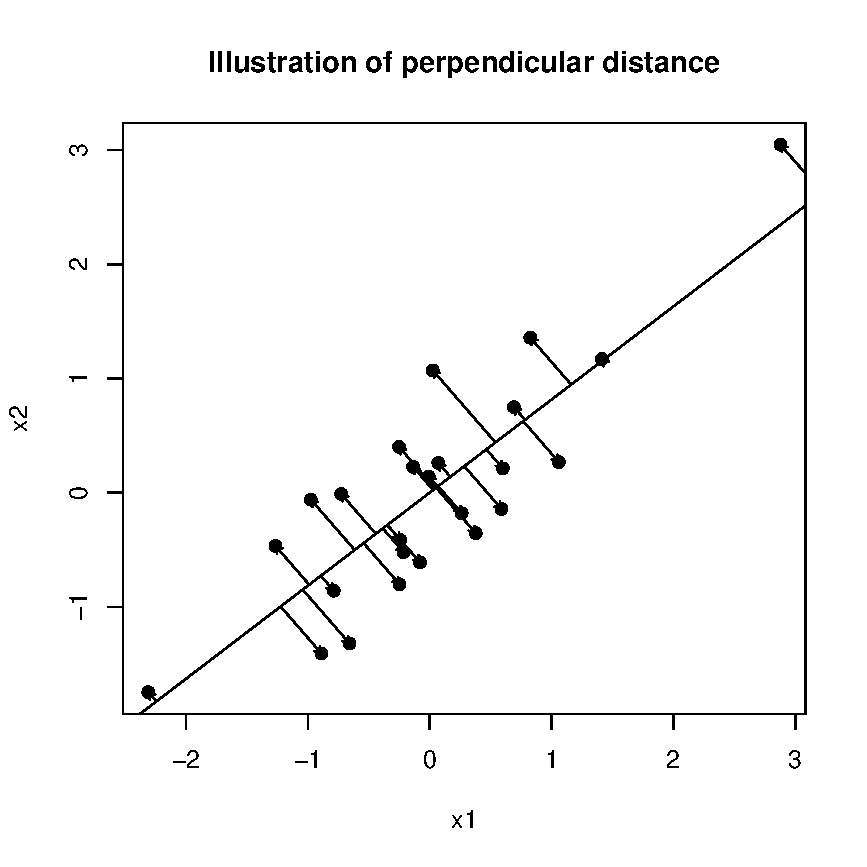
\includegraphics[width = 0.7\textwidth]{images/ProjDist}
\caption{Illustration of perpendicular distance}
\label{projection}
\end{figure}

\singlespacing
\begin{verbatim}
require(MASS)
X <- scale(mvrnorm(25, c(2,2), matrix(c(1,0.8,0.8,1),2,2)))
eqscplot(X)
X.cov <- cov(X)
X.ed <- eigen(X.cov)
proj <- X.ed$vec[,1] %*% t(X.ed$vec[,1])
y <- t(proj %*% t(X))
abline(a=0,b=X.ed$vec[2,1]/X.ed$vec[1,1])
arrows( X[,1], X[,2], y[,1],y[,2], length = 0.05, col = "green")
\end{verbatim}
\onehalfspacing

Plotting the ordinary least squares solutions is easy enough, although when regression X[,1] on X[,2] the gradient needs to be inverted (or the axes reversed).

\singlespacing
\begin{verbatim}
## plot the ols of X[,2] on X[,1]
eqscplot(X)
X2.lm <- lm(X[,2] ~ X[,1])
abline(X2.lm, col = "red", lwd = 2)
arrows(X[,1],X[,2], X[,1], predict(X2.lm),  length = 0.01, col = "red")
points(X[,1],X[,2], pch = 16)
## plot the ols of X[,1] on X[,2]
eqscplot(X)
X1.lm <- lm(X[,1] ~ X[,2])
abline(0, 1/coef(X1.lm)[2], col = "blue")## need to invert the gradient
arrows(X[,1],X[,2], predict(X1.lm), X[,2],  length = 0.01, col = "blue")
points(X[,1],X[,2], pch = 16)
\end{verbatim}
\onehalfspacing


It is informative to contrast the line plotted in figure \ref{projection} with those produced by linear regression of $x$ on $y$ as well as $y$ on $x$.
The matrix $ \boldsymbol{a} \boldsymbol{a}^{T} $ can be referred to as the projection matrix.   

\subsection{Principal Component Stability}
\label{sec:pcastability}

Whilst considering the geometry, it is useful to motivate some ideas about the differences between population and sample principal components by simulating three datasets from the same parameters.   For population 1, we draw from standard normal variables with correlation of 0.9, for population 2 the variables are uncorrelated.   In other words, $\boldsymbol{\mu}_{1} = \boldsymbol{\mu}_{2} = (0,0)^{T}$, $\boldsymbol{\Sigma}_{1} = \left(\begin{array}{rr} 1 & 0.9 \\ 0.9 & 1 \end{array} \right)$ but $\boldsymbol{\Sigma}_{2} = \left(\begin{array}{rr} 1 & 0 \\ 0 & 1 \end{array} \right)$

Simulating the data is simple enough, for example:
\singlespacing
\begin{verbatim}
X <- mvrnorm(100, c(0,0), matrix(c(1,.9,.9,1),2,2))
V <- var(X)
eV <- eigen(V)
\end{verbatim}
\onehalfspacing

\singlespacing
\begin{verbatim}
plot(X, xlim = c(-3,3), ylim = c(-3,3))
abline(a=0,b=eV$vec[2,1]/eV$vec[1,1])
abline(a=0,b=eV$vec[2,2]/eV$vec[1,2])
\end{verbatim}
\onehalfspacing

Just so the eigenvalues don't feel left out, we can add constant density ellipses to these plots, details on these were given in \ref{cdellipse}.  Essentially, we can define a constant density ellipse from the ``centre'' as $\pm c \sqrt{\lambda_{i}} \boldsymbol{\alpha}_{i}$, here we take $c=1.96$.   In the code snippet below, \verb+x+ and \verb+y+ are the coordinates of an ellipse scaled from a unit circle by the two eigenvalues.   These are then rotated by the angles of the eigenvectors:

\singlespacing
\begin{verbatim}
theta <- seq(0,(2*pi),length=101)
x <- 1.96 * sqrt(eV$val[1]) * cos(theta)
y <- 1.96 * sqrt(eV$val[2]) * sin(theta)
newxy <- cbind(x,y) %*% t(eV$vec)
lines(newxy)
\end{verbatim}
\onehalfspacing

We now consider figure \ref{pcastabsynth}, which overlays three samples from each of the two populations specified.   The semi-major axis, the contribution to the first principal component has been denoted with solid lines, the semi-minor axis, the contribution to the second principal component, has been denoted by dotted lines.   It should be very apparent that there is some variation in the orientation of the axes, as might be expected the eigenanalysis varies slightly according to sample properties.   However, the right hand side of the plot is intended to illustrate the problem of sphericity.   Without a strong correlation structure, the angles subtended by the principal components varies massively.

\begin{figure}
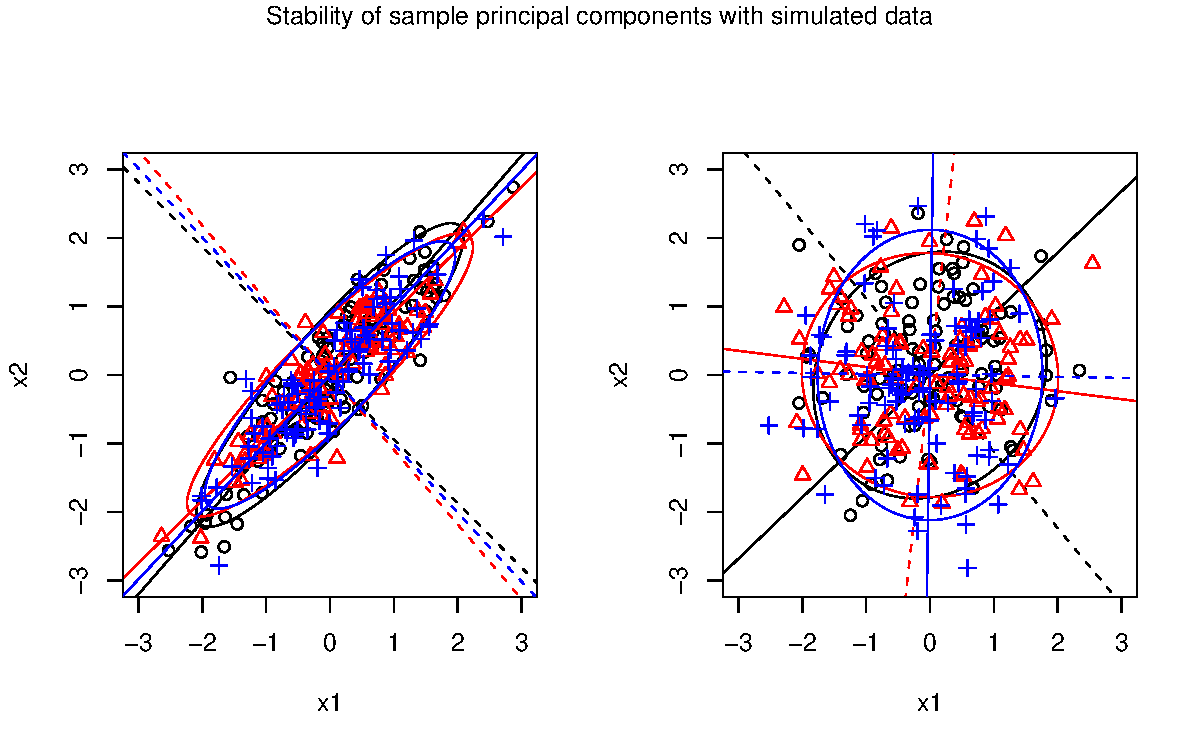
\includegraphics[width = 0.9\textwidth]{images/pcastability}
\caption{Artificially generated data indicating stablity of pca solution}
\label{pcastabsynth}
\end{figure}

Whilst this is an artificial example in many senses (not only are the data simulated but we have only two variables), but the problem is an important one.   In particular, when exploring dimension reduction properties of principal components we have to be attendant to the possibility of partial sphericity; that some of the $q+1, \ldots, p$ principal components essentially exhibit this behaviour.   We consider specific hypothesis tests for this problem later.


Finally, whilst talking about projections, we make one comment in relation to projection pursuit.   This technique will be considered further in the next chapter.   Suffice to say here that projection pursuit is a generic set of techniques which aims to find ``interesting'' projections of data.   The user decides on the dimensionality of the projection and selects a suitable criterion of interestingness.  \cite{Bolton+Krzanowski:1999} give results interpreting principal components analysis within this framework, the criterion (projection pursuit index) in this case is given by:

\begin{displaymath}
I = max(\boldsymbol{e} \boldsymbol{S} \boldsymbol{e}^{T}); \boldsymbol{e}\boldsymbol{e}^{T}=1,
\end{displaymath}
where $\boldsymbol{S}$ is the sample covariance matrix.   This index is the minimum of the maximised log-likelihood over all projections when normality is assumed.

However, they go on to imply that more ``interesting'' projections are less likely to have normally distributed data by showing that in terms of the likelihood$\mathscr{L}(\boldsymbol{e})$, this decreases as $\boldsymbol{e} \boldsymbol{S} \boldsymbol{e}^{T}$ increases.  Assuming the usual maximum likelihood estimators for $\boldsymbol{\mu}$ and $\boldsymbol{\Sigma}$:
\begin{eqnarray*}
\mathscr{L}(\boldsymbol{e}) &=& max \mathscr{L} (\boldsymbol{x}; \boldsymbol{\mu}, \boldsymbol{\Sigma}, \boldsymbol{e})\\
&=& - \frac{n}{2} \left[ p + p \log \left(\frac{2 \pi n}{n-1}\right) \right] - \frac{n}{2} \log |\boldsymbol{e} \boldsymbol{S} \boldsymbol{e}^{T}|
\end{eqnarray*}
In other words, under normality, the most ``interesting'' projection is the one with the maximised likelihood.


\section{Some properties of principal components}

Before considering some examples of principal component analysis we first consider a number of fundamental properties.


\begin{definition}
\label{def:princomp}
If $\boldsymbol{x}$ is a mean centred random vector, with covariance matrix $\boldsymbol{\Sigma}$, the principal components are given by:
\begin{equation}
\boldsymbol{x} \rightarrow \boldsymbol{z} = \boldsymbol{E}^{T}(\boldsymbol{x} - \boldsymbol{\mu})
\end{equation}
i.e. the transformation requires mean-centred variables.   $\boldsymbol{E}$ is orthogonal, $\boldsymbol{E}^{T}\boldsymbol{\Sigma}\boldsymbol{E}$ is diagonal, $\lambda_{1} \geq \lambda_{2} \geq \ldots \geq \lambda_{p} \geq 0$ provided $\boldsymbol{\Sigma}$ is positive definite.
\end{definition}

A number of key propeties immediately follow from their derivation from the spectral decomposition:


\begin{theorem}
\begin{equation} 
\label{pcszero}
\mbox{E}(z_{i}) = 0
\end{equation}

\begin{equation}
\mbox{Var}(z_{i}) = \lambda_{i}
\end{equation}
hence:
\begin{equation}
\mbox{Var}(z_{1}) \geq \mbox{Var}(z_{2}) \geq \ldots \geq \mbox{Var}(z_{p});
\end{equation}
in particular it should be noted that no standardised linear combination of $\boldsymbol{x}$ has a larger variance than $\boldsymbol{\lambda}$.

We finally restate the implications of finding orthogonal projections.
\begin{equation}
\mbox{Cov}(z_{i},z_{j}) = 0, i \neq j;
\end{equation}

\end{theorem}


One property we will make repeated use of concerns the proportion of variance explained by each principal component:

\begin{theorem}
\label{th:eigentrace}
The trace of a covariance matrix is equal to the sum of its eigenvalues:
\begin{equation}
\label{eigentrace}
trace(\boldsymbol{\Sigma}) = \sum_{i=1}^{p} \lambda_{i}
\end{equation}
\end{theorem}

In other words, equation~\ref{eigentrace} indicates that the \emph{total variance} can be explained by the sum of the eigenvalues.   In the case of principal components formed from the correlation matrix $\boldsymbol{R}$ this will be equal to the number of variables.


\begin{theorem}
\label{th:eigenproduct}
The generalised variance (the determinant of a covariance matrix) can be expressed as the product of its eigenvalues:
\begin{equation}
\lvert \boldsymbol{\Sigma} \rvert = \prod_{i = 1}^{p} \lambda_{i}
\end{equation}
\end{theorem}
Theorem \ref{th:eigenproduct} indicates that we can find an estimate of the \emph{generalised variance} from the product of the eigenvalues.   Along with theorem \ref{th:eigentrace} we find that the generalised variance and the sum of variances are unchanged by the principal component transformation.   

Finally, a note is needed on scale-invariance.   \cite{Flury:1997} describes this last as an anti-property.   Principal components are not-invariant to changes of scale.   Standardising variables is rather a brutal way of dealing with this.   Explanations are given in most multivariate textbooks, for example both formal and information explanaitions are given by [page 219] \cite{Mardia+etal:1979}.   Nevertheless, if variables are recorded on widely differing scales, a principal component analysis of the covariance matrix will largely reflect the variables with the numerically greatest variance.   It is therefore important that the variables are in some sense comparable; this can either be achieved by standardising, or by some gentler transformation.   We will find that the heptathalon data has to be standardised, whereas it is possible to take logs of the turtle data.


Finally, we consider one important property, which is more in the \cite{Pearson:1901} sense.   

\begin{theorem}
The first $k$ principal components have smaller mean squared departure from the population (or sample) variables than any other $k$-dimensional subspace.
\end{theorem}
Proof: [page 220] \cite{Mardia+etal:1979}

This property is rather important when considering the dimension reducing properties of principal component as it does not require any distributional assumptions.



\section{Illustration of Principal Components}

 We define the sample principal components by $\boldsymbol{e}$ and $\ell$.

Having now hopefully explained the rationale behind principal components analysis, we consider some illustrative analysis before considering further inferential developments.

\subsection{An illustration with the Sydney Heptatholon data}

Before doing anything else with these data, it needs to be noted that in the three running events, better performance is indicated by a lower measure (time), whereas in the jumping and throwing events good performance is indicated by a higher measure (distance).   It seems sensible to introduce a scale reversal so that good performance is in some way at the top of any given scale.   A convenient way of doing this is to multiply the times of the running events by $-1$.

\singlespacing
\begin{verbatim}
hept.df <- read.csv("Heptatholon.csv", row.names = 1)
hept.df$X100mHurdles.S. <- hept.df$X100mHurdles.S. * -1
hept.df$X200m.sec. <- hept.df$X200m.sec. * -1
hept.df$r800m.s. <- hept.df$r800m.s. * -1
\end{verbatim}
\onehalfspacing

These variables are clearly incomparably in any sense.    It is also clear that we need to work with the correlation matrix for these data, there is considerable difference in the scales (running 800 metres tends to take rather longer than running 100 metres).   We will also centre the variables using \verb+scale()+ which saves us a little work later on.  

\singlespacing
\begin{verbatim}
hep.scale <- scale(hept.df[,-1])
hept.cormat <- cor(hept.df[,-1])
hep.ev <- eigen(hept.cormat)
\end{verbatim}
\onehalfspacing

Our principal component analysis then basically consists of extracting \verb+hep.ev$values+ contains the eigenvalues, and \verb+hep.ev$vectors+ contains the eigen vectors.   Our first set of loadings are given by the first row of the eigenvectors, we can form the first linear combination:

\singlespacing
\begin{verbatim}
> hep.ev$vectors[,1]
> z1 <- hep.scale %*% hep.ev$vectors[,1]
\end{verbatim}
\onehalfspacing

in a similar manner it is possible to form $z_{2}$ and so on.  


This means that the proportion of total variance explained by each linear combination can be given by $\frac{\lambda_{i}}{ \sum_{i=1}^{p} \lambda_{i}}$
, which can be calculated for our heptathalon data with \verb+hep.ev$values/sum(hep.ev$values)+.   It is also conventional to produce a ``scree'' plot of this information with something like \verb+plot(hep.ev$values, type = "b")+ which graphically represents the amount of variance explained by each linear combination.

%par(las = 1)
%plot(hep.ev$values, type = "b", main = "Scree plot from Heptathalon data", ylab = "Variance explained", xlab = "Principal component", pch = 16)


\begin{figure}
\begin{center}
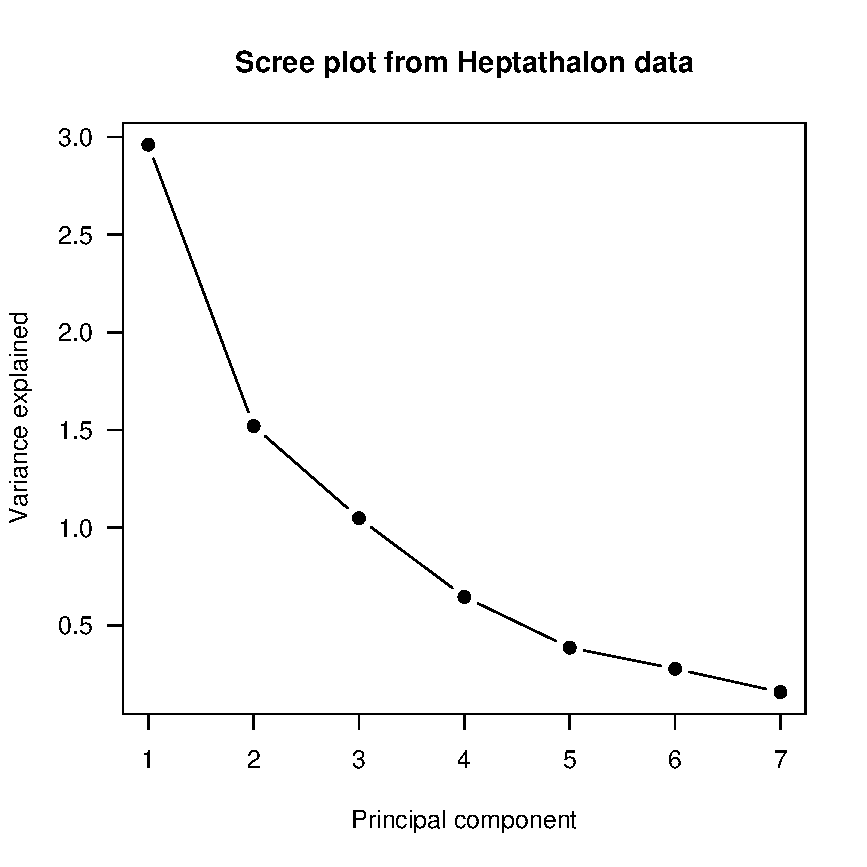
\includegraphics[width = 0.5\textwidth]{images/HeptathScree} 
\caption{Scree plot displaying the amount of variation explained by each of the seven principal components formed from the correlation matrix of the Sydney Heptathalon data}
\label{screeplot}
\end{center}
\end{figure}


\subsection{Principal component scoring}

As stated at the start of the chapter, the principal component scores are essentially derived from the mean centered data.   

In other words, we found:

\begin{equation}
\label{pcascore}
\boldsymbol{z} =  \boldsymbol{E}^{T}(\boldsymbol{x}-\boldsymbol{\mu})
\end{equation}

It is possible (although somewhat unusual in this context) to find scores from the standardised data

\begin{equation}
\boldsymbol{z} =  \boldsymbol{E}^{T}(\boldsymbol{x}-\boldsymbol{\mu})  \boldsymbol{\Lambda}^{-1/2}
\end{equation}

It should be noted that \cite{Rencher:2002} really doesn't approve of this latter effort, it essentially leaves us looking at the correlation between the standardised data and the principal component scores.   We therefore consisder the more usual scores given in equation \ref{pcascore}.   The first four eigenvectors are given as follows:

\singlespacing
\begin{verbatim}
$vectors
           [,1]        [,2]        [,3]         [,4]
[1,] -0.4656494  0.28868133  0.32883275 -0.003922038  
[2,] -0.2455859 -0.56442826 -0.10737271 -0.610427608  
[3,] -0.4195748 -0.07137064 -0.52173345  0.235891780 
[4,] -0.4330174 -0.02204083  0.51825157  0.357022268 
[5,] -0.4630436  0.11516723  0.12459693 -0.480637087 
[6,] -0.3228125  0.38161226 -0.56832241  0.091073036 
[7,] -0.2017272 -0.65849286 -0.03216966  0.452710298 
\end{verbatim}
\onehalfspacing

So to find the first principal component we only need to compute the following:

\begin{displaymath}
z_{i1} = a_{11} x_{i1} + a_{12} x_{i2} + a_{13} x_{i3} + \ldots
\end{displaymath}

which means that the first principal component can be given as:

\begin{displaymath}
Z_{i1} = -0.4656 \times x_{1} - 0.2456 \times x_{2} - 0.4196 \times x_{3} + \ldots
\end{displaymath}

Clearly this can also be calculated as matrix product $\boldsymbol{X}\boldsymbol{a}$.

\singlespacing
\begin{verbatim}
hep.ev$vectors[,1] ## first vector of pc loadings
scores <- hep.scale %*% hep.ev$vectors
par(mfrow = c(3,3))
apply(scores, 2, qqnorm)
scoresR <- hep.scale %*% (hep.ev$vectors %*% diag(hep.ev$values^-0.5))
\end{verbatim}
\onehalfspacing

If we wished, we can carry out further investigation of the principal component scores.


\subsection{Prepackaged PCA function 1: \texttt{princomp()}}

In practice it will come as no surprise to learn that there are prepackaged functions in \textbf{R} for carrying out a principal components analysis.   \verb+princomp()+ has been provided for comparability with S-Plus.  We will find out later that the preferred function uses the singular value decomposition.   However, there are good reasons for examining \verb+princomp()+ first.    It is based on carrying out an eigen decomposition, by default of the covariance matrix and it should be noted that the covariance matrix esimated by \verb+cov.wt+ uses the divisor $N$, rather than the unbiased version $N-1$.    It is possible to supply robust estimates of the covariance matrix via \verb+covmat+, this does allow a form of robust principal components and as we work through the heptathalon data we will find out that this may indeed be useful.  
It is possible to call \verb+princomp()+   with the specification \verb+cor=TRUE+ to use the sample correlation matrix rather than sample covariance matrix.

The main results can be accessed via \verb+summary()+ and \verb+print()+.   The eigenvectors are extracted and printed with a degree of pretty printing using \verb+loadings()+.   If necessary, the square roots of the eigenvalues (i.e. the standard deviations of each principal component) are stored within the princomp object and can be extracted manually using \verb+$sdev+.   The principal component scores themselves can be accessed via \verb+$scores+ if these have been requested.    There are also graphical methods associated with \verb+princomp()+ objects, \verb+plot()+ produces a screeplot, \verb+biplot()+ produces a biplot, we explain this tool further in section~\ref{prcomp}.   However, we note an important aspect of eigenanalysis, which is very clearly stated in the helpfile and will be quite important later:
\begin{quote}
The signs of the columns of the loadings and scores are arbitrary, and so may differ between different programs for PCA, and even  between different builds of R.
\end{quote}
This is a point we will return to a few times particularly when considering bootstrapping!

Executing a principal component analysis is therefore trivial, as demonstrated in the following code snippet.   We extract the principal component scores and create qq plots; as demonstrated in chapter 2 any univariate linear combination of multivariate normal data should be normally distributed.  

\singlespacing
\begin{verbatim}
hept.princomp <- princomp(hept.df[,-1], scale = TRUE)
summary(hept.princomp)
plot(hept.princomp) ## produces scree plot
par(mfrow = c(3,3))
apply(hept.princomp$scores, 2, qqnorm)
\end{verbatim}
\onehalfspacing


\subsection{Inbuilt functions 2: \texttt{prcomp()}}
\label{prcomp}

The preferred \textbf{R} function for a conventional principal component analysis is \verb+prcomp()+.   There are a number of differences in use and extraction, but the rather more important difference is that it is based upon a singular value decomposition of the data.   The singular value decomposition was outlined in Section~\ref{svd}.   Whilst discussing the singular value decomposition in this context it is convenient to introduce the biplot.   \cite{Gabriel:1971} introduced the biplot as a means of representing either a matrix of rank two, or a rank two approximation to a matrix of rank greater than two.   The idea is to display vectors for each row and vectors for each column are displayed on the same plot, illustrating features of either a rank two matrix or a rank two approximation.   Whilst we illustrate it in detail here, it has application in areas other than with principal components.

As discussed earlier, we consider data matrix $\boldsymbol{X}$; it's decomposition is given by:
\begin{displaymath}
\boldsymbol{X} = \sum_{i=1}^{p} \lambda_{i} \boldsymbol{u}_{i} \boldsymbol{v}_{i}^{T}
\end{displaymath}
and hence for the biplot, where we specifically require a rank two solution:
\begin{displaymath}
\boldsymbol{X} = \sum_{i=1}^{2} \lambda_{i} \boldsymbol{u}_{i} \boldsymbol{v}_{i}^{T} = 
\left( \boldsymbol{u}_{1},  \boldsymbol{u}_{2} \right) 
\left( \begin{array}{cc} \lambda_{1} & 0 \\ 0 & \lambda_{2} \end{array} \right) \left( \begin{array}{c} \boldsymbol{v}_{1}^{T} \boldsymbol{v}_{2}^{T} \end{array} \right)
\end{displaymath}

Based on this decomposition, we have a choice of plots.   In general, we can plot:
\begin{displaymath}
\boldsymbol{g}_{i}^{T} = \lambda_{1}^{1-\zeta} u_{1i}, \lambda_{1}^{1-\zeta} u_{2i}
\end{displaymath}
for the observations
and
\begin{displaymath}
\boldsymbol{h}^{T}_{j} = \lambda_{1}^{\zeta} q_{1j} \lambda_{2}^{\zeta} q_{2j}
\end{displaymath}
for the columns.
where $0 \leq \zeta \leq 1$.   \cite{Gabriel:1971} essentially gave proposals for $\zeta = 0$, $\zeta = 0.5$ and $\zeta = 1$.   In \textbf{R}, these can be set with the argument \verb+scale+ which takes the range $0 \leq \mbox{scale} \leq 1$.   The default is \verb+scale = 1+ which implies $\boldsymbol{H}^{T}\boldsymbol{H} = \boldsymbol{I}$; more notably this means that the inner products between variables approximate covariances and distances between observations approximate Mahalanobis distance.    By default, observations are scaled up by $\sqrt{n}$, variables are scaled down by $\sqrt{n}$

It is possible to adjust \verb+choices=c(1,2)+ if you don't really want a biplot but want to examine the projection of what are in this context other principal components.


\singlespacing
\begin{verbatim}
pairs(turtles[,-1],
   lower.panel = function(x, y){ points(x, y,
   pch = unclass(turtles[,1]),
   col = as.numeric(turtles[,1]))},
   main = "Pairwise scatter plots for painted turtles")
\end{verbatim}
\onehalfspacing

We follow \cite{Flury:1997} in transforming these data onto the log scale (and multiplying them by 10).   This is quite common in allometric applications, where the $\log$ transformation may suffice in terms of bringing all variables onto a comparable scale.

\singlespacing
\begin{verbatim}
data(turtles)
  turtles.m <- subset(turtles, turtles$Gender == "Male")
  turtles.m <- 10 * log(turtles.m[,-1])
  turtles.m.prcomp <- prcomp(turtles.m)
  summary(turtles.m.prcomp)
plot(turtles.m.prcomp)
turtles.m.prcomp$sdev^2 ## extract eigenvalues
par(xpd = NA)
biplot(turtles.m.prcomp)
\end{verbatim}
\onehalfspacing

%turtles.prcomp <- prcomp(turtles[,-1])
%plot(turtles.prcomp$x[,1], turtles.prcomp$x[,2],
% col = as.numeric(turtles[,1]),
% pch = as.numeric(turtles[,1]))

We can illustrate the biplot as follows by carrying out the various computations by hand within \textbf{R}:

\singlespacing
\begin{verbatim}
turtles.svd <- svd(turtles.m)
H <- cbind(turtles.svd$u[,1], turtles.svd$u[,2]) * sqrt(24)
g1 <- turtles.svd$d[1] * turtles.svd$v[,1] / sqrt(24)
g2 <- turtles.svd$d[2] * turtles.svd$v[,2] / sqrt(24)
plot(H)
par(new = TRUE)
plot(c(-arrx,arrx),c(-arry,arry), type = "n",
  xaxt = "n", yaxt = "n")
axis(3)
axis(4)
arrows(0, 0, arrx, arry)
\end{verbatim}
\onehalfspacing


\section{Principal Components Regression}

Finally, we say a few words about principal components regression, and illustrate the use of principal components in bioinformatics with the superpc package.


\section{``Model'' criticism for principal components analysis}

This section has deliberately given a provocative title.   ``Model'' criticism clearly requires some kind of model, it is worth giving some thought to whether we are using a principal components model in the context of a model or not.   It is possible to use the technique as a data analytical technique, particularly when used for data reduction there is no necessity to assume multivariate normality.   However, when we are using it in the context of a multivariate normal distribution, it is important to be aware of a number of key distributional results on the asymptotic distribution of the eigenvalues and eigenvectors of a covariance matrix.


\subsection{Distribution theory for the Eigenvalues and Eigenvectors of a covariance matrix}

\cite{Girshink:1939,Anderson:1963} give results for asymptotic distributions in connection with the covariance matrix.   Firstly, we comment on the existence of maximum likelihood estimators for the eigendecomposition of a covariance matrix:

\begin{theorem}
\label{th:evalmle}
Under conditions of normality, the maximum likelihood estimators for the population eigenvalues and eigenvectors of $\boldsymbol{\Sigma}$ are given by the sample eigenvalues and eigenvectors, provided all the eigenvalues are distinct.
\end{theorem}
Proof: See [page 229] \cite{Mardia+etal:1979} and [page 460] \cite{Anderson:1984}



Theorem \label{th:evalmle} indicates that our sample eigenvalues are the maximum likelihood estimators of their corresponding population counterparts.   In most inferential situations we would wish to qualify such an estimator with guidance as to the level of associated uncertainty.   Firstly, we wish to establish the distribution of the eigenvalues.

\begin{theorem}
\label{th:pcasymptotics}
The asymptotic distribution of eigenvalues and eigenvectors can be expressed as follows:
\begin{equation}
\label{pcasymptotics}
\sqrt{n}(\boldsymbol{\ell} - \boldsymbol{\lambda}) \sim MVN(\boldsymbol{0}, 2\boldsymbol{\Lambda}^{2})
\end{equation}
%\begin{equation}
%\sqrt{n} \frac{\mathscr{l}_{i} - \lambda_{i}}{\sqrt{2}\mathscr{l}_{i}} \to^\infty N(0,1)
%\end{equation}
where $\Lambda$ is the diagonal matrix of eigenvalues.   This can be expressed equivalently as:
\begin{equation}
\label{pcaasymptoticslog}
\sqrt{n}\left(\log(\boldsymbol{\ell}) - \log(\boldsymbol{\lambda})\right) \sim MVN(\boldsymbol{0}, 2)
\end{equation}

 and 
\begin{equation}
\sqrt{n}(\hat{\boldsymbol{e}}_{i} - \boldsymbol{e}_{i}) \sim MVN(\boldsymbol{0}, \boldsymbol{E}_{i})
\end{equation}
where $\boldsymbol{E}_{i} = \lambda_{i} \sum_{k = 1, k \neq i}^{p} \frac{\lambda_{k}}{(\lambda_{k} - \lambda_{i})^{2}} \boldsymbol{e}_{k}\boldsymbol{e}^{T}$
\end{theorem}
Proof: The proof for this has been restated in \cite{Flury:1988}.   These properties were established following work by \cite{Anderson:1963} and \cite{Girshink:1939}.


Theorem \ref{pcasymptotics} indicates that for large $n$, the eigenvalues $\lambda_{i}$ are independently distributed.   We can therefore obtain standard errors for the eigenvalues as follows:
%\subsection{Confidence intervals for the eigenvalues and eigenvectors}
%\label{pcaconfint}
\begin{displaymath}
se(\lambda_{j}) = \sqrt{2/n} \lambda_{j},
\end{displaymath}
giving confidence intervals:
\begin{displaymath}
\frac{\ell_{i}}{1 + \sqrt{2/n} z_{\alpha/2}} \leq \lambda_{i} \leq \frac{\ell_{i}}{1 + \sqrt{2/n} z_{1-\alpha/2}}
\end{displaymath}
and the standard error for the corresponding eigenvectors are given by: 
\begin{displaymath}
se(\alpha) = \left( \frac{1}{n} \lambda_{j} \sum_{j+1; j \neq h}^{p} \frac{\lambda_{j}}{(\lambda_{j} - \lambda_{h})^2} \alpha_{jh}^{2} \right)^{1/2}.
\end{displaymath}


We can illustrate calculation of these standard errors, as well as estimation of associated confidence intervals by adapting code written by Marco Bee  to accompany \cite{Flury:1997}).   This code will be set out at an S3 class in \textbf{R}.   Firstly therefore, we set out a container:
\singlespacing
\begin{verbatim}
lpc <- function(X){
  UseMethod("lpc", X)
}
\end{verbatim}
\onehalfspacing

And now we can write out a default method which calculates the relevant confidence intervals:
\singlespacing
\begin{verbatim}
lpc.default <- function(X)
{
n <- dim(X)[1]; p <- dim(X)[2]  # number of observations 
X.prcomp <- prcomp(X)
evals <- X.prcomp$sdev^2 
Ones <- matrix(1, p, p) 
Lambda <- Ones * evals
Q <- (t(Lambda) - Lambda + diag(p))^(-2) - diag(p) # nifty trick
Theta1 <- sweep(Q, 2, evals, FUN="*") 
Theta <- Theta1 * evals # compute matrix of theta-coefficients
stdeB <- matrix(0,p,p)      
   h <- 1
      while (h <= p){ 
      V <- X.prcomp$rotation %*% 
          (Theta[, h] * t(X.prcomp$rotation))  
      stdeB[, h] <- sqrt(diag(V)/n)
      h <- h + 1 
      }                         
stdelam <- sqrt(2/n) * evals
results <- list("eigenvectors" = X.prcomp$rotation, 
  "eigenvalues" = X.prcomp$sdev^2,
  "stdeB" = stdeB, "stdelam" = stdelam)
  class(results) <- "lpc"
  results
}
\end{verbatim}
\onehalfspacing

Having returned the standard error we can write a simpler print function which displays the eigenvectors and eigenvalues along with their associated standard error:
\onehalfspacing
\begin{verbatim}
print.lpc <- function(x) {
print(x[1]) ## eigenvectors
print(x[2]) ## eigenvalues
cat("standard errors for eigenvector coefficients:")
print(x[3])
cat("standard errors for eigenvalues:")
print(x[4])
cat("\n\n")
invisible(x)
}
\end{verbatim}
\onehalfspacing

So for example, with the turtles data:
\singlespacing
\begin{verbatim}
> lpc(subset(turtles, turtles$Gender == "Male")[,-1])
$eigenvectors
          [,1]        [,2]        [,3]
[1,] 0.8401219  0.48810477 -0.23653541
[2,] 0.4919082 -0.86938426 -0.04687583
[3,] 0.2285205  0.07697229  0.97049145

$eigenvalues
[1] 195.274633   3.688564   1.103833

standard errors for eigenvector coefficients:$stdeB
           [,1]       [,2]       [,3]
[1,] 0.01442666 0.04469703 0.07885419
[2,] 0.02487011 0.01592627 0.13874655
[3,] 0.01513963 0.15478836 0.01276277

standard errors for eigenvalues:$stdelam
[1] 56.370931  1.064797  0.318649

\end{verbatim}
\onehalfspacing

And if we wanted to estimate the confidence intervals we can write an associated \verb+summary+ method which will do the additional calculations and return the results.   Note in the code below that we have allowed for a \emph{Bonferroni} adjustment.   If we wish to adjust for making $m$ comparisons we can replace $z_{\frac{\alpha}{2}}$ with $z_{\frac{\alpha}{2m}}$  

\singlespacing
\begin{verbatim}
summary.lpc <- function(x, alpha = 0.05, bonferroni = FALSE) {
if (!is.null(alpha)){ ## calculate ci if asked
  if (bonferroni == TRUE) {alpha = alpha / length(x[[2]])}
  z <- abs(qnorm((1-alpha)/2))
}
print(x[1]) ## eigenvectors

if (!is.null(alpha)){
cat(round(alpha * 100), "\% CI: \n ")
veclo <- x[[1]] - z * x[[3]]
vechi <- x[[1]] + z * x[[3]]
print(veclo)
print(vechi)
cat("\n")
} 

print(x[2]) ## eigenvalues

if (!is.null(alpha)){
cat(round(alpha * 100), "\% CI: \n ")
vallo <- x[[2]] - z * x[[4]]
valhi <- x[[2]] + z * x[[4]]
print(vallo)
print(valhi)
cat("\n")
} 

cat("standard errors for eigenvector coefficients:")
print(x[3])

cat("standard errors for eigenvalues:")
print(x[4])
cat("\n\n")
invisible(x)
}
\end{verbatim}
\onehalfspacing

%This should place some cautions on arbitrary cutoffs, e.g. Kaiser.


\section{Sphericity}
\label{Sphericity}

We preface this section on sphericity with some results concerning covariance / correlation matrices which are of less than full rank.   If a symmetric positive definite matrix (correlation and covariance matrices are at least semi-definite).   If such a matrix is of full rank $p$ then all the eigen values are positive.   
%If the matrix is of rank $m < p$ then there will be $m$ positive eigenvalues and $p-m$ zero eigenvalues.   We will consider this sphericity problem in some detail later.
%We preface comments on sphericity with one point concerning the rank of the covariance or correlation matrix.   
If the rank of the covariance or correlation matrix $m < p$ then the last $p-m$ eigenvalues are identically zero.   The converse of this theorem is that any non-zero eigen value can be considered to be \emph{significantly} non-zero.

However, we are now going to consider sphericity, where there are not $p$ distinct eigenvalues.   We highlighted earlier the potential problem of sphericity and the effect on a resultant principal component analysis.
Clearly there is little point carrying out a principal component analysis under conditions of sphericity.   We can consider three possiblilites, where $\boldsymbol{R} = \boldsymbol{I}$, which can arise either because $\boldsymbol{S} = s \boldsymbol{I}$ or the more general possibility that $\boldsymbol{S}$ is diagonal.


We firstly consider the most general possibility, that $\boldsymbol{\Sigma} \propto \sigma \boldsymbol{I}$ where $\sigma$ is unspecified.   However, this test is equivalent to examining whether all the roots of $|\boldsymbol{\Sigma} - \lambda \boldsymbol{I}| = 0$ are equal.   In this eventuality, the arithmetic and geometric means will be identical

We firstly consider a general test for sphericity proposed by \cite{Mauchly:1940}


\begin{theorem}
We consider that:
\label{th:sphericity}
\begin{displaymath}
\frac{\prod_{j=1}^{p} \lambda_{i}^{1/j}}{\sum_{j=1}^{p} \lambda_{i}^{1/j}} = \frac{\lvert \boldsymbol{\Sigma} \rvert^{1/j}}{\frac{1}{j} tr(\boldsymbol{\Sigma})}
\end{displaymath}

This yields the following test statistic.   Under the null hypothesis $H_{0}: \boldsymbol{S} = \sigma \boldsymbol{I}$, the test statistic $m$ given by:
\begin{equation}
m = \frac{\lvert \boldsymbol{S} \boldsymbol{\Sigma}_{0}^{-1} \rvert^{n/2}}
{ \left[ \frac{1}{p} trace(\boldsymbol{S} \boldsymbol{\Sigma}_{0}^{-1} )^{pn/2} \right] } 
\end{equation}
\end{theorem}


This is pre-implemented in \textbf{R} for manova type objects, therefore if we fit a null manova object we can carry out this test:

\singlespacing
\begin{verbatim}
obj <- manova(as.matrix(turtles.m) ~ 1)
mauchly.test(obj)

        Mauchly's test of sphericity

data:  SSD matrix from manova(as.matrix(turtles.m) ~ 1) 
= 101.1821, p-value < 2.2e-16
\end{verbatim}
\onehalfspacing

And so we have evidence (provided the test assumptions are met) that the turtle data are not spherical.


For completeness, we mention here another test for sphericity is given by [see section 1.9] \cite{Morrison:2005} based upon the determinant of the correlation matrix.

\begin{definition}
\label{morrison}
Under the null hypothesis $H_{0}: \boldsymbol{R} = \boldsymbol{I}$, the test statistic $w$ given by:
\begin{displaymath}
w = -\left( n - \frac{2p + 5}{6} \right) \log \lvert \boldsymbol{R} \rvert
\end{displaymath}
has a $\chi^{2}$ distribution with $\frac{1}{2}p(p-1)$ degrees of freedom.
\end{definition}

This test is quite simply coded up in \textbf{R}.

\singlespacing
\begin{verbatim}
morrison <- function(data){
  n <- dim(data)[1]; p <- dim(data)[2];
  wnm <- -(n - (2 * p)/6) * log(det(cor(data)))
    cat(paste("wnm = ", wnm, "\n"))
    cat(paste("df = ", p * (p - 1) * 0.5, "\n"))
    cat(paste("Chisq density = ", dchisq(wnm, p * (p - 1) * 0.5) , "\n"))
}
\end{verbatim}
\onehalfspacing

Again, this test confirms non-sphericity of the Turtles data.

\subsection{Partial sphericity}

It is usually the case that partial sphericity is or more practical concern than more complete independence of the data.   We will consider more heuristic methods for selecting the dimensionality of a principal component projection later, but clearly the eigenvectors of principal components with equal eigenvalues are too poorly defined to be of any practical use.   We are therefore interested in partial sphericity, where $\lambda_{q+1} = \lambda_{q+2} = \ldots = \lambda_{p}$

%We highlighted in theorem \ref{pca:lowrank} that whenever the covaraiance matrix had rank $r<p$ there were $r$ principal components.   More notably, we highlighted the problem in \label{sec:pcastability} of sphericity.   In practice, we may be more concerned about partial sphericity; whilst the first $q$ eigenvalues are distinct we may be concerned that the smallest eigenvalues, $q+1, \ldots, p$, are equal.   

Where we have partial sphericity, we may note the following theorem:

\begin{theorem}
For normal data, where the eigenvalues of $\boldsymbol{\Sigma}$ are not distinct then the m.l.e. of $\bar{\lambda}$ is the corresponding arithmetic mean of the sample eigenvalues, and the corresponding eigenvectors are maximum likelihood estimators although they are not unique.
\end{theorem}
Proof: See \cite{Anderson:1963}

The asymptotic theory set out above leads to a number of possible tests for partial sphericity.   One likelihood ratio can be considered as follows:

\begin{definition}

[page 198] \cite{Seber:1984} gives a likelihood ratio test for partial sphericity.   In order to determine whether whether the last $p-q$ eigenvalues are equal can be specified as follows.   We wish to test $H_{0}: \lambda_{q+1} = \lambda_{q+2} = \ldots = \lambda_{p}$ versus $H_{a}: \lambda_{q+1} > \lambda_{q+2} > \ldots > \lambda_{p}$.

\begin{equation}
-2 \log \mathscr{l} = - n \log \left( \prod_{q=1}^{p} \frac{\lambda_{j}}{\bar{\lambda}} \right)
\end{equation}
where $\bar{lambda} = \frac{1}{p-q} \sum_{j=q}^{p} \lambda_{j}$.   Under the null hypothesis, the likelihood ratio statistic, $-2 \log \mathscr{l}$, of the eivenvalues derived from a covariance matrix is distributed as $\chi^{2}_{\frac{1}{2}(p-q-1)(p-q+2)}$.  The test can be applied to the correlation matrix but the asymptotic distribution is no longer chi-square.   The asymptotics can be improved with a correction proposed by \cite{Lawley:1956}:

%this uses Anderson:1963 and Fujikoshi:1978 asymptotics on chisq.

\begin{equation}
- \left\{ n - 1 - q - \frac{2(p-q)^{2} + (p-q) + 2}{6(p-q)} + \sum_{j=1}^{q} \left(\frac{\bar{\lambda}}{\lambda_{j} - \bar{\lambda}} \right)^2 \right\}  \log \left( \prod_{q=1}^{p} \frac{\lambda_{j}}{\bar{\lambda}} \right)
\end{equation}

This test is however not robust to departures from normality.


%\label{th:sphertest}
%The likelihood ratio test for the hypothesis $\lambda_{q+1} = \cdots = \lambda_{p}$ versus the alternative $\lambda_{q+1} > \cdots \lambda_{p}$ is given by:

%\begin{equation}
%\varphi(q, p-q) = N(p-q) 
%\frac{\frac{1}{p-q} \sum_{j=q=1}^{p} \lambda_{j}}
%{(\prod_{j=q=1}^{p} \lambda_{j} )^{1/(p-q)}}
%\end{equation}
%\end{theorem}
%Proof: \cite{Anderson:1984}

%$\varphi \sim \chi_{((p-q)((p-q)+1)/2 - 1)}^{2} as N \rightarrow \inf$

%It is therefore possible to test for sphericity of a $q$ dimensional solution, increasing this by one and not worrying about the multiple testing problem.

\end{definition}

It is reasonably straightforward to start coding a function to execute this in \textbf{R}, a sketch of such a function is illustrated here:
\singlespacing
\begin{verbatim}
spher <- function(X, q){
  p <- dim(X)[2]; n <- dim(X)[1]; r <- p-q
  X.prcomp <- prcomp(X)
  evals <- X.prcomp$sdev^2
  retain <- evals[1:q]; discard <- evals[-(1:q)]
  lambdahat <- mean(discard)
  bit <- sum(lambdahat / (retain - lambdahat) )^2
  corr <- n - 1 - q - (2 * r^2 + r + 2)/(6*r) + bit
  product <- prod(discard / lambdahat)
  lrt <- -corr * log(product)
  df <- 0.5 * (r-1) * (r+2)
    cat(paste("-2log L = ", lrt, "\n") )
    cat(paste("df = ", df, "\n") )
    cat(paste("Chisq density ", dchisq(lrt, df ), "\n" ))
    ##return(lrt)
}
\end{verbatim}
\onehalfspacing

We illustrate this with the turtle data.   Recalling that the first eigenvalue was 2.33, considerably greater than the second and third eigenvalues of 0.06 and 0.036.

\singlespacing
\begin{verbatim}
> spher(turtles.m, 1)
-2log L =  1.34290454195737 
df =  2 
Chisq density  0.255482988814162 
\end{verbatim}
\onehalfspacing

So in this case we cannot reject $H_{0}$ and have no evidence that the second and third eigenvalues are distinct.   We might be included to consider the possibility here that that $\lambda_{2} = \lambda_{3}$ and would therefore be somewhat wary of the resultant eigenvectors.


A simpler explanation is given in [page 622] \cite{Flury:1997}, which follows from that given in [page 475] \cite{Anderson:1984}, and is given in slightly different form in [page 235] \cite{Mardia+etal:1979}.%##mkb <- n* p * (a - 1 - log(g) ) ##mkb pg 235
This relies on a log likelihood statistic derived as a ratio of arithmetic to geometric means of the eigenvalues.

\singlespacing
\begin{verbatim}
function(X, q){
  p <- dim(X)[2];  n <- dim(X)[1];  r <- p-q
  X.prcomp <- prcomp(X)
  evals <- X.prcomp$sdev^2
  q1 <- q+1
    discard <- evals[q1:p]
    a <- sum(discard) / r
    g <- prod(discard)^(1/r)
    s <- n * r * log(a / g)
    df <- 0.5 * r * (r+1)
  cat(paste("-log L = ", s, "\n") )
  cat(paste("df = ", df, "\n") )
  cat(paste("Chisq density ", dchisq(lrt, df ), "\n" ))
  ##return(s)
}
\end{verbatim}
\onehalfspacing

Asymptotically, this value can be considered to follow a $\chi^{2}_{\frac{1}{2}(p-q)(p-q+1) - 2}$ distribution under the null hypothesis.   It can be seen that is related to the test of complete sphericity.   This test can be used with the turtle data and again confirms the possible that the second and third principal components can be considered spherical and should not be interepreted further.


%Yet another likelihood ratio test exists for this.

%\begin{displaymath}
%\Lambda = \frac{|\boldsymbol{S}|^{n/2}}{\prod s_{ij}^{n/2}} = |\boldsymbol{R}|^{n/2} < c
%\end{displaymath}
%$-2 \log \Lambda \sim \chi^{2}$ with Bartlett continuity corrections

%In the case of the latter, $\lambda = 1 + (p-1) \rho$, eigenvectors = $\frac{1}{\sqrt{p}}$


\subsection{High Dimensional Tests for Sphericity}

Having (hopefully) demonstrated the importance of sphericity in conventional principal components analysis we refer to results which carry out analagous procedures in high dimensions.   Whilst the asymptotic tests above rely on $n \to \infty$, it can be problematic where $p > n$.   More recent work therefore examines how one might carry out tests for this eventually.   We firstly consider testing whether $\boldsymbol{\Sigma} \propto \boldsymbol{I}$ 

\begin{theorem}
A test for $\boldsymbol{\Sigma} \propto \boldsymbol{I}$ which is reliable whenever $p > n$ can be given as follows:
\begin{equation}
U = \frac{1}{p} trace \left( (\frac{\boldsymbol{S}}{(1/p)trace(\boldsymbol{S})} - \boldsymbol{I} )^{2} \right)
\end{equation}
In this case, it may be noted that $\frac{np}{2} U$ asymptotically follows a $\chi^{2}$ distribution with $\frac{1}{2}p(p+1)-1$ degrees of freedom. 

Proof: See \cite{Ledoit+Wolf:2002}, following work by \cite{John:1971,John:1972}
\end{theorem}

This can be very simply estimated in \textbf{R}:

\singlespacing
\begin{verbatim}
JohnsU <- function(data){
  p <- dim(data)[2]
  S <- cov(data)
  traceS <- sum(diag(S))
  traceSI <- sum(diag(S-diag(rep(1, p))))
    u <- 1/p * traceS / (1/p*traceSI^2)
    test <- n * p * 0.5 * u
    df <- (0.5 * p * (p+1)) - 1
  cat(paste("U = ", test, "\n") )
  cat(paste("df = ", df, "\n") )
  cat(paste("Chisq density ", dchisq(test, df ), "\n" ))
}
\end{verbatim}
\onehalfspacing

So we can estimate the sphericity quite simply

\singlespacing
\begin{verbatim}
JohnsU(khan$train)
\end{verbatim}
\onehalfspacing

Which appears to indicate little evidence for sphericity.

Testing the correlation matrix is not quite so straighforward to expansion of $p$ relative to $n$.    $\boldsymbol{\Sigma} = \boldsymbol{I}$

\begin{theorem}
A test for $\boldsymbol{\Sigma} = \boldsymbol{I}$ which is reliable whenever $p > n$ is given by:
\begin{equation}
\label{ledoit}
W = \frac{1}{p} trace \left\{ \left( \boldsymbol{S} - \boldsymbol{I} \right)^{2} \right\} - \frac{p}{n} \left\{ \frac{1}{p} trace(\boldsymbol{S}) \right\}^{2} + \frac{p}{n}
\end{equation}
Under $H_{0}$, assuming multivariate normality $\frac{nm}{2} W \rightarrow ^{d} \chi^{2}_{p(p+1)/2-1}$

Proof: \cite{Ledoit+Wolf:2002}
\end{theorem}

\singlespacing
\begin{verbatim}
ledoitwolf <- function(data){
  n <- dim(data)[1]; p <- dim(data)[2] 
  S <- cor(data)
  traceS <- sum(diag(S))
  SI <- crossprod(S - diag(rep(1, p)))   
  traceSI <- sum(diag(SI))
    w <- 1/p*traceSI - p/n*(1/p*traceS)^2 + p/n
    test <- n * p * 0.5 * w
    df <- (0.5 * p * (p+1))
  cat(paste("U = ", test, "\n") )
  cat(paste("df = ", df, "\n") )
  cat(paste("Chisq density ", dchisq(test, df ), "\n" ))
}
\end{verbatim}
\onehalfspacing


However, we can consider results based on those indicated in  \ref{morrison} which can be used to test whether $\boldsymbol{R} = \boldsymbol{I}$.  

\begin{theorem}
A test statistic for sphericity is given by:
\begin{displaymath}
t = \sum_{i=2}^{p} \sum_{j=1}^{i-1} r_{ij}^{2} - \frac{p(p-1)}{2n}
\end{displaymath}
Which is asymptotically normal with zero mean and variance:
\begin{displaymath}
\sigma_{t}^{2} = \frac{p(p-1)(n-1)}{n^{2}(n+2)}
\end{displaymath}
Proof: See \cite{Schott:2005}
\end{theorem}


This is simply illustrated in \textbf{R}.

\singlespacing
\begin{verbatim}
schott <- function(data){
  n <- dim(data)[1]; p <- dim(data)[2]
  R <- cor(data)
  R[lower.tri(R) == FALSE] <- NA
  red <- na.omit(as.vector(R))
   tnm <- sum(red^2) 
   cf <- (p * (p-1)) / (2 * n)
   test <- tnm - cf
   sigma2 <- (p * (p-1) * (n-1)) / (n^2 * (n+2) )
  cat(paste("tnm = ", tnm, "cf = ", cf,  "\n") )
  cat(paste("Normal density ", dnorm(test, sqrt(sigma2) ), "\n" ))
}
\end{verbatim}
\onehalfspacing

Again, a call to \verb+schott(khan$train)+ confirms that these data are non-spherical.

As before, perhaps we are more interested in the generalisations of these statistics, i.e. we are concerned with partial sphericity and wish to determine whether the smallest $p-q$ eigenvalues of $\boldsymbol{\Sigma}$ are equal.

\begin{theorem}
Generalising equation \ref{ledoit}, a test for partial sphericity can be based upon the following test statistic:
\begin{equation}
u = \frac{ (1/p) \sum_{i=q+1}^{p} \lambda_{i}}{\left[(1/p) \sum_{i=q+1}^{p} \lambda_{i} \right]^{2}} - 1
\end{equation}
where $\frac{n-q}{u}$\footnote{check this} can be compared with a $\chi^{2}$ distribution with $p(p+1)/2 - 1$ degrees of freedom.     
\end{theorem}
Proof: \cite{Schott:2006}

Again, this test can be coded up in \textbf{R} and examined in the context of the khan data.

\singlespacing
\begin{verbatim}
schottpartial <- function(X, q){
  p <- dim(X)[2]; n <- dim(X)[1]; r <- p-q
  X.prcomp <- prcomp(X)
  evals <- X.prcomp$sdev^2
  discard <- evals[-(1:q)]
  u <- (sum(discard^2) / r) / (sum(discard) / r)^2  - 1
  df <- 0.5 * r * (r+1) - 1
    cat(paste("u = ", u, "\n") )
    cat(paste("df = ", df, "\n") )
    cat(paste("Chisq density ", dchisq(u * (n-q), df ), "\n" ))
    ##return(lrt)
}
\end{verbatim}
\onehalfspacing




It is bearing in mind that just because the smallest $p-q$ eigenvalues indicate the corresponding principal components explain very little of the variation, they do not necessarily contain any useful information.


%library(made4)
%data(khan)
%khan.coa<-ord(khan$train, classvec=khan$train.classes, type="pca")  
%khan.coa$ord$eig
%dim(khan$train)


%\begin{displaymath}
%U_{r} \left( \frac{
%\frac{1}{r}  sum_{i+q+1}^{p} \lambda_{i}^{2} }
%{(\frac{1}{r} sum_{i+q+1}^{p} \lambda)^{2}} - 1 \right)
%\end{displaymath}
%where $r = p-q$, i.e. we are looking for a test to reject the $r$th smallest eigenvalues.   It can be shown that testing $(n-q) U_{r} > \chi^{2}_{\frac{r(r+1)}{2}-1, 1-\alpha}$, where $\alpha$ is the required significance level and 



\section{How many components to retain}

We have considered formal hypothesis testing for sphericity and partial sphericity.   This may well indicate that it is not sensible to include a number of principal components in a given representation of multivariate data.   However, we may not really be interested in modelling multivariate normality.   We may not like asymptotics.   We will consider a few further results on selecting the number of principal components in any given projection of the data.

Whilst principal components have optimality properties in terms of providing the best lower dimensional projection in terms of mean squared error.   Nevertheless, they are often used, however informally, in an inferential role.   Consideble care is needed in their interpretation.   It is important to note that we are working with sample principal components, these can be somewhat unstable relative to the puted underlying population components.   It makes little sense to attempt anything resembling inferential work without considering the stability of a particular principal component solution.   Typically, having decided how best to scale the data, the next most important question surrounds how many components need to be retained.   We will first consider some of the more informal procedures used to guide this judgement, and will subsequently consider methods derived from normal theory inference.



\subsection{Data analytic diagnostics}

A number of proposals have been made in the literature concerning decisions surrounding the ``number of components'' to retain.  The following are some of the more popular proposals:

%\begin{itemize}
%\item Retaining enough components to explain more than x\% of the variation, where x has been determined \textit{a priori} and is in the order of 80 or 90\%.
%\item Looking for a change in the slope of the scree plot - the last components where the line flattens are usually discarded
%\item Interpreting the scree plot in the presence of monte carlo simulations
%\item Retaining all components explaining an above average amount of variation (i.e. in the case of components derived from the correlation matrix this is all components with an eigenvalue above 1)
%\item Broken stick approach
%\item Using the empirical distribution function, i.e. bootstrapping
%\end{itemize}


\subsection{Proportion of variance explained}
\label{propexpl}

The proportion of variance explained is a rather informal method for selecting $q$, the number of dimensions in the principal component projection required to adequately explain the data.   Essentially, one decides \textit{a priori} that a certain amount of variance is to be explained, and only accepts solutions meeting that requirement.   It is however consistent with the exploratory nature to which principal component analysis is often applied.


We can however, using the asymptotic theory set out above, develop a confidence interval for the proportion of variance explained.   %We suggested in section \ref{propexpl} that one might choose the dimensionality of the solution based on whether it meets some predetermined arbitrary proportion of variance.  We have confidence intervals for these values as well.

\begin{theorem}
\label{th:propexpl}

We denote our estimate of the proportion of variation explained by $\pi$:
\begin{displaymath}
\pi = f(\lambda) = \frac{ \sum_{i=1}^{q} \lambda_{i} }{ \sum_{i=1}^{p} \lambda_{i} }.
\end{displaymath}

If we also consider the corresponding sum of squares:
\begin{displaymath}
\zeta = \frac{\sum_{i=1}^{q} \lambda_{i}^{2}}{ \sum_{i=1}^{p} \lambda_{i}^{2}}
\end{displaymath}

Under conditions of multivariate normality, we can obtain an estimate of the variance associated $\pi$, the proportion of variance explained as follows:
\begin{equation}
\eta^{2} = \frac{2 trace(\Sigma)}{(n-1)  (trace(\Sigma))^{2}} = \pi^{2} - 2 \zeta \pi + \zeta^{2}
\end{equation}
\end{theorem}
\textbf{Proof}: \cite{Sugiyama+Tong:1976} and [page 454] \cite{Kshinaragar:1972}

Hence we can derive a confidence interval for $\pi$ as follows.

This can be illustrated as follows:

\singlespacing
\begin{verbatim}
vals <-  hep.ev$values^2
q <- 3
alpha <- 0.95
alpha <- 1 - (1-alpha)/2

pi <- sum(vals[1:q]) / sum(vals)
alpha <- sum(vals[1:q]^2) / sum(vals^2)## by vector recycing
eta2 <- pi^{2} - 2 * alpha * pi + alpha^2
cat(pi, eta2)
cat("\n")
cat(pi + qnorm(alpha)*eta2)
cat("\n")
cat(pi - qnorm(alpha) * eta2)
cat("\n")
\end{verbatim}
\onehalfspacing





\subsection{Change in slope of the scree plot}
\label{screeslope}

\cite{Cattell:1966} proposed the scree plot in the context of (principal component extracted) factor analysis.   Without wishing to add to the confusion between the two techniques, it has become a fairly standard technique for assessing the adequacy of a number of dimension reducing techniques.   Both \texttt{prcomp} and \texttt{princomp} objects have a plot method which yields a scree plot, the idea is to select components up to the point where the slope changes direction.

\singlespacing
\begin{verbatim}
plot(hept.princomp)
\end{verbatim}
\onehalfspacing

\subsection{Interpreting the scree plot in the presence of simulations}
\label{screemc}

It is possible to extend the basic scree plot idea.   \cite{Horn:1965} suggested simulating data from a multivariate normal having the same sample size, the same number of variables, the same means and variances but having zero covariances.   There are a couple of manifestations of this approach within various \textbf{R} packages, for example \verb+psy+ package contains a ready made function.   The scree plot of with zero correlation is expected to be a straight line, it can be compared with the scree plot from the observed data.   It is possible to extend this to a full Monte Carlo test, the code listing below goes someway towards this.

\singlespacing
\begin{verbatim}
Horn <- function(data, reps){
p <- dim(data)[2]
n <- dim(data)[1]
Varmat <- matrix(0,p,p)
Mean <- mean(data)
diag(Varmat) <- diag(var(data))

Evals <- princomp(data, cor = TRUE)$sdev^2
idx <- barplot(Evals, names.arg = paste("PC", c(1:7)), 
xlab = "Component", ylab = "Proportion of trace", 
main = "Proportion of trace explained")

results <- matrix(0,reps,p)
  for (i in 1:reps){
  SimData <- mvrnorm(n, Mean, Varmat)
  ExpEvalsH <- princomp(SimData, cor = TRUE)$sdev^2
  results[i,] <- ExpEvalsH
  lines(idx, ExpEvalsH, type = "b", pch = 16)
  }

lines(idx, apply(results, 2, mean), type = "b", col = "red")

legend("topright", lty = 1, pch = 16, legend = "Expected values")
Results <- data.frame(Evals = Evals, ExpEvalsH = ExpEvalsH)
}

Horn(hept.df[-1], 10)
\end{verbatim}
\onehalfspacing

\includegraphics[width = 0.7\textwidth]{images/Horn}


\subsection{Broken Stick}
\label{brokenstick}

Another approach to assessing the proportion of variation explained has been made by \cite{Jolliffe:1986} who suggests using a ``broken stick'' approach.   The idea here is that if any unit is randomly divided into $p$ segments, the expected length of the $k$th longest segment is:
\begin{equation}
\label{stick}
l_{k} = \left(\frac{1}{p} \right) \sum_{i=k}^{p} \left( \frac{1}{i} \right)
\end{equation}
If we assume that the total variance, $trace{\boldsymbol{S}} = \sum_{j=1}^{p}$, is the ``stick'', we can use this approach to estimate an expected size of each eigenvalue.   A rather simple function to calculate the expected values indicated by \ref{stick} is given below, the expected values are plotted alongside the observed values from a \texttt{princomp()} object created from the Heptathalon data.   It should be noted that \texttt{princomp()} returns the standard deviations (\verb+$sdev+), these have therefore been squared to recoved the eigenvalues $\lambda_{i}$.

\singlespacing
\begin{verbatim}
> stickometer <- function(p){
  vec <- 1 / (1:p)
  stick <- vector("numeric", p) 
  stick[1] <- sum(vec)
     for (i in 2:p){
     stick[i] <- sum(vec[-(1:(i-1))])}
  stick <- 1/p * stick
  names(stick) <- paste("Comp.", c(1:p), sep = "")
  return(stick)
}
> 
> stick <- stickometer(7)
> proptrace <- hep.princomp$sdev^2 / sum(hep.princomp$sdev^2)
>
> stick
> proptrace
> 
> idx <- barplot(proptrace, names.arg = paste("PC", c(1:7)), 
> xlab = "Component", ylab = "Proportion of trace", 
> main = "Proportion of trace explained")
> lines(idx, stick, type = "b", pch = 16)
> legend("topright", lty = 1, pch = 16, legend = "Expected values")
\end{verbatim}
\onehalfspacing

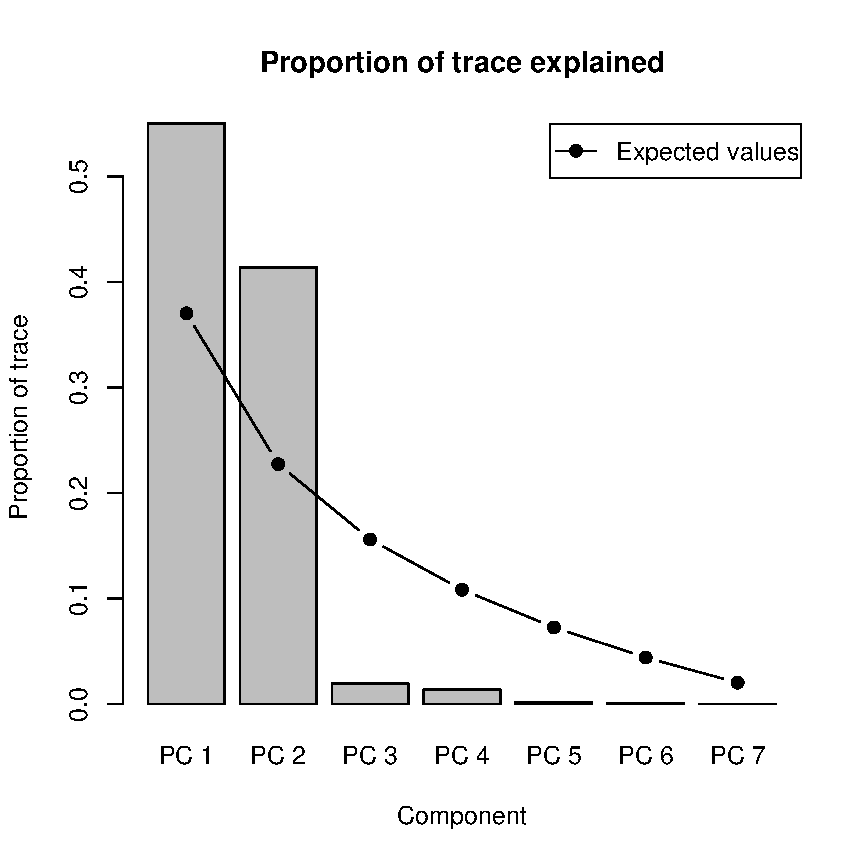
\includegraphics[width = 0.7\textwidth]{images/stick}

Examination of the results (numbers or the plot) suggest that the first and seventh components are accounting for slightly more variation than would be expected purely by chance.

\subsection{Kaiser Criterion}
\label{kaiser}

The Kaiser Criteria is a rather inflexible criteria widely met in many sofware packages.   Basically it amounts to retaining all components where the eigenvalue is greater than the mean of the eigenvalues.   In the case of principal components based on the correlation matrix this clearly means retaining all components where the eigenvalue is greater than one.  Whilst one may not wish to assume multivariate normality, the asymptotics considered next provide a clear warning that population eigenvalues greater than one could clearly be realised in a sample with values below one.


Karlis provide some caveats on the use of this criteriosn.

\subsection{Cross validation}

Cross-validation in the context of principal components was proposed by \cite{Wold:1976,Wold:1978} and developed by \cite{Eastment+Krzanowski:1982}.   In essence, the sample can be randomly split into $g$ groups, the loadings can be estimated from reduced sets omitting each of the $g$ groups in turn, but the predicted values can be found from these $g$ groups using the loadings estimated from the other rows.   The value for $(\boldsymbol{\hat{x}} - \boldsymbol{x})$ can be estimated from equation \ref{Qstats}, and the PRESS statistic estimated.


\singlespacing
\begin{verbatim}
pcaxv <- function(X){
  UseMethod("pcaxv", X)
}
\end{verbatim}
\onehalfspacing

It is useful to create an \texttt{S3} object to carry out this procedure.   The working function is given by:

\singlespacing
\begin{verbatim}
pcaxv.default <- function(X, g = 5){
    N <- dim(X)[1]
    p <- dim(X)[2]
      index <- sample(c(1:N) )
      groups <- gl(g, N %/% g)
         Q <- matrix(0, g, p)
           for (i in 1:g){
           dot <- prcomp(X[-index[groups == i],])
         Q[i,] <- colSums((as.matrix(scale(X))[index[groups == i],]
                       %*% dot$rotation)^2)}
    colmeans <- colSums(Q) / N
  PRESS <- cumsum(colmeans[c(p:1)])/ c(1:p)
  PRESS <- PRESS[c(p:1)]
  names(PRESS) <- paste("C", c(0:(p-1)))
  results <- list("PRESS" = PRESS, 
    dm = pcaxvconstants(N,p)$dm, dr = pcaxvconstants(N,p)$dr)
class(results) <- "pcaxv"
results
}
\end{verbatim}
\onehalfspacing

The function \verb+pcaxvconstants()+ calculates some constants that can be used in the summary function.   A suitable print function for use with cross-validation objects created here can be given as follows:

\singlespacing
\begin{verbatim}
print.pcaxv <- function(x){
cat("Components Removed \n")
  print(x[[1]])
  cat("\n")
  invisible(x)
}
\end{verbatim}
\onehalfspacing

[page 354] \cite{Jackson:1991} refers to a $W$ statistic (without giving any idea as to its origin or distribution.   The idea behind this $W$ statistic however is that for any component where $W > 1$ we have evidence to retain the component, where $W < 1$ we have an adequate representation of our data swarm without that component.   The constants calculated earlier are basically $D_{M} = n + p - 2(p-q)$, $D_{R} = p (n - 1) - \sum_{i=1}^{(p-q)}(n + p - 2i)$, and $W$ is given by:

\begin{equation}
W = \frac{ (PRESS((p-q)-1) - PRESS(p-q))/D_{M}(p-q)}{PRESS(p-q)/D_{R}(p-q)}
\end{equation}

\singlespacing
\begin{verbatim}
summary.pcaxv <- function(x){
  cat("PRESS for components Removed \n")
  print(x[[1]])
  cat("\n")
    wl <- length(x$PRESS)-1
    w <- rep(NA, wl)
       for (i in 1:wl){
       w[i] <- ((x$PRESS[i] - x$PRESS[i+1]) / x$dm[i+1] ) / 
             (x$PRESS[i+1] / x$dr[i+1] ) }
    names(w) <- paste("C", c(1:wl))
  cat("W for components included \n")
  print(w)
invisible(x)
}
\end{verbatim}
\onehalfspacing


These are rather interesting concepts in practice.   For example, considering the \verb+turtle+ data examined earlier:

\singlespacing
\begin{verbatim}
> turtle.xv <- pcaxv(as.matrix(log(turtles[,-1])))
> turtle.xv
PRESS for components Removed 
       C 0        C 1        C 2 
0.97916667 0.05952219 0.06118754 

W for components included 
        C 1         C 2 
29.00900476 -0.02605895 
\end{verbatim}
\onehalfspacing

Which appears to provide strong evidence that the turtle data can be represented by one principal component.

One little glurp can happen with the $W$ statistic.   Consider the water strider data given in \cite{Flury:1997}.

\singlespacing
\begin{verbatim}
data(strider)
dot <- pcaxv(as.matrix(log(strider)))
summary(dot)
PRESS for components Removed 
       C 0        C 1        C 2        C 3        C 4        C 5 
0.98863636 0.27912037 0.23714880 0.15109046 0.10068831 0.05974256 

W for components included 
       C 1        C 2        C 3        C 4        C 5 
11.8809534  0.6686066  1.6310744  0.9662281  0.6690516 
\end{verbatim}
\onehalfspacing

It can be seen that the second component has a $W$ below 1, but for the third is clearly above 1, and for the fourth is is very close to 1.   \cite{Jackson:1991} suggests that this may be due to the presence of outliers - this is left as an exercise for further examination.


The following functions (a) need tidying up and (b) support the pcaxv function - they're left here for tidiness only;

\singlespacing
\begin{verbatim}
rtota <- function(N, p, q){
  rtot <- 0
  for (i in 1:q){
  rtot <- rtot + N + p - 2 * i
  }
rtot
}


pcaxvconstants <- function(N,p){
  dm <- N + p - 2 * (p - c(p:1))
  dm[1] <- NA
    dr <- rep(0,p)
    dr[1] <- p * (N-1)
  for (i in 2:p){
  dr[i] <- p * (N - 1) - rtota(N, p, i-1)
}
results <- list(dm = dm, dr = dr)
}
\end{verbatim}
\onehalfspacing



\subsection{Bootstrapping}
\label{bootstrap}

We discuss standard errors derived from asymptotic theory in the next section, but clearly there are limitations in having to assume multivariate normality.   Bootstrapping avoids any such assumptions, we can make inference based upon an empirical distribution function.   For tidiness, we will make a little function that calls \texttt{prcomp()} and returns the eigenvalues and eigenvectors only:

\singlespacing
\begin{verbatim}
theta <- function(x.data, x){
eta <- prcomp(x.data[x,])
return(cbind(eta[[1]], eta[[2]]))
}
\end{verbatim}
\onehalfspacing

However, whilst computer power might be cheap, nothing in life is free and the problem with eigenvectors is the arbitrariness of the signs.   Accordingly, it is completely unacceptable to use bootstrapping without checking for inversions of eigenvectors.   Below we consider carrying out some boostrapping, plot the results and identify the most unreasonably volatile eigenvector.   We can use the sign of this eigenvector to adjust the signs of all the other components of this eigenvector and hence obtain bootstrap estimates of the eigenvectors.

Then we call the function with our data, and tell it how many sets of bootstraps we want:

\singlespacing
\begin{verbatim}
> library(boot)
> hep.boot <- boot(hep.scale, theta, R = 50, sim = "ordinary")
> eigen.bootplot(hep.boot,8,7)
\end{verbatim}
\onehalfspacing

\begin{figure}
\begin{center}
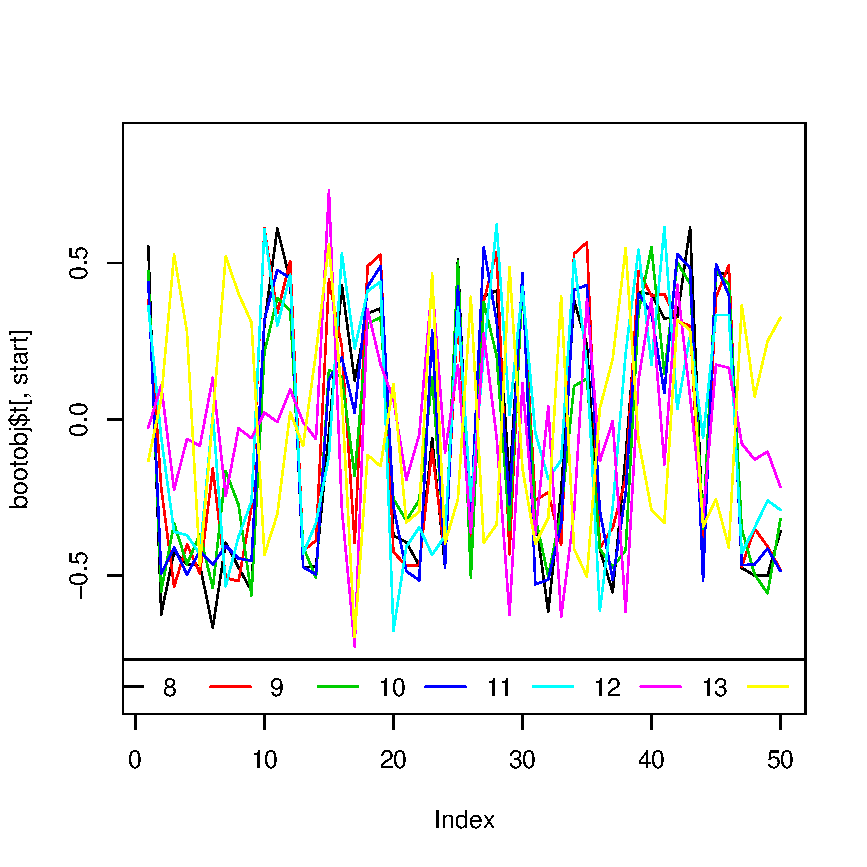
\includegraphics[width = 0.7\textwidth]{images/boottraceplot}
\caption{Trace of bootstrap iterations for first eigenvector}
\label{boottrace}
\end{center}
\end{figure}

It is quite clear that we need to invert some eigenvectors.   One approach is to identify one coefficient within an eigenvector and whenever this is below zero to multiply the entire vector by the scalar -1.   

\singlespacing
\begin{verbatim}
> idx <- hep.boot$t[,8] < 0
> hep.boot$t[idx,c(8:14)] <- hep.boot$t[idx,c(8:14)] * -1
> eigen.bootplot(hep.boot,8,7)
\end{verbatim}
\onehalfspacing

In this way we can obtain additional information on the variability of our principal component analysis.




\subsection{Other structure matrices}


We might also be interested in testing for other structure matrices, such as equi-correlation.   See \cite{Lawley:1963}.

\begin{eqnarray*}
\bar{r}_{k} = \frac{1}{p-1} \sum_{i=1; i \neq k}^{p} r_{ik}; k = 1, \ldots, p\\
\bar{r} = \frac{2}{p(p-1)} \sum_{i<k} \sum r_{ik}\\
\hat{alpha} = \frac{(p-1)^{2} \left[ 1 - (1 - \bar{r})^{2} \right] }{
p - (p - 2)(1 - \bar{r})^{2}}
\end{eqnarray*}

where $\frac{n-1}{(1-\bar{r})^{2}} \alpha$ follows a $T^{2}$ distribution.

Proof: JW 489  

\begin{verbatim}
mean(spot[lower.tri(spot)])
\end{verbatim}




\subsection{Forward search}

A more recent proposal for assessing the stability of principal component solution is the forward search \cite{Atkinson+etal:2004}.


\subsection{Assessing multivariate normality}
\label{mahalpca}

If we are prepared to entertain the idea that our data might be multivariate normal, it is very simple to obtain distance measures from the principal component scores and examine the adequacy of a representation in this context (clearly this might not be so useful if we are cannot assume multivariate normality).   Given a random vector $\boldsymbol{x}$ having mean $\boldsymbol{\mu}$ and covariance matrix $\boldsymbol{\Sigma}$, \cite{Flury:1997} (page 608-609) demonstrates the relationship between the principal component scores $z_{j}$ and the mahalanobis distance $\delta^{2}(\boldsymbol{x}, \boldsymbol{\mu})$ (which he calls the squared standard distance).   

\begin{theorem}
\begin{equation}
\label{Qstats}
\delta^{2}(\boldsymbol{x}, \boldsymbol{\mu}) = (\boldsymbol{x} -  \boldsymbol{\mu}) \boldsymbol{\Sigma}^{-1} (\boldsymbol{x} -  \boldsymbol{\mu}) = \sum_{j=1}^{p} \frac{z_{j}^{2}}{\lambda_{j}}
\end{equation}
where $\boldsymbol{z} = (z_{1}, \ldots, z_{p})^{T} = \boldsymbol{E}(\boldsymbol{x}- \boldsymbol{\mu})$, and $\boldsymbol{\Sigma} = \boldsymbol{E \Lambda E}^{T}$ as above.   
\end{theorem}
Proof: See \cite{Flury:1997}

We can use our principal component representation to partition the mahalanobis distance.   We want $\delta_{a}^{2} =  \sum_{j=1}^{q} \frac{z_{j}^{2}}{\lambda_{j}}$ corresponding to the distance encapsulated in our first $q$ principal components, and $\delta_{b}^{2} =  \sum_{j=q+1}^{p} \frac{z_{j}^{2}}{\lambda_{j}}$ corresponding to the distances encapsulated by the last $(p-q)$ principal components.   \cite{Flury:1997} indicates that these can be represented by $\chi^{2}$ random variables with respectively $q$ and $p-q$ degrees of freedom which lends itself to diagnostic assesment of the adequacy of the principal component representation.   It should perhaps be noted that this is a large sample approximation, \cite{Gnanadesikan:1977} (page 172) suggests $n = 25$ is adequate in the bivariate case.   \cite{Bilodeau+Brenner:1999} (page 186) therefore indicate the use of the Beta distribution, with $\alpha = \frac{p-2}{2p}$ and $\beta = \frac{n - p - 2}{2(n - p - 1)}$.   


It is possible to write a simple function to extract the distances associated with accepted and rejected principal component (and the total distance) which can then be used in various diagnostic plots.

\singlespacing
\begin{verbatim}
> princomp2dist <- function(obj.princomp, retain){
 scores <- t(t(obj.princomp$scores^2) / obj.princomp$sdev)
 dtot <- apply(scores, 1, sum)
 d1 <- apply(scores[,c(1:retain)], 1, sum)
 d2 <- apply(scores[,-c(1:retain)], 1, sum)
 dists <- data.frame(dtot = dtot, d1 = d1, d2 = d2)
 return(dists)
}

> hept.princomp <- princomp(hept.df[-1], scores = TRUE, scale = TRUE)
> ## form a princomp object
> hept.m <- princomp2dist(hept.princomp, 3)
> ## extract distances based on 3 component representation
\end{verbatim}
\onehalfspacing

Having obtained the distances, we only need some suitable method of investigation.   The most useful are qq-plots.   Given we have only 26 rows and 9 columns, we will use a modified verion of the \texttt{qqbeta} function given by \cite{Bilodeau+Brenner:1999}.   This plots the Mahalanobis distance against a suitable beta distribution.

\singlespacing
\begin{verbatim}
> qqbetaM <- function(x, p) {
  n <- length(x)
  a <- p/2
  b <- (n-p-1)/2
  alpha <- 0.5*(a-1)/a
  beta <- 0.5*(b-1)/b
  x <- sort(x)
  y <- qbeta(((1:n)-alpha)/(n-alpha-beta+1),a,b)*(n-1)^2/n
  plot(x,y,xlab="Mahalanobis distances",ylab="Beta quantiles")
}
> qqbetaM(hept.m$dtot,  7)
\end{verbatim}
\onehalfspacing

\begin{figure}
\begin{center}
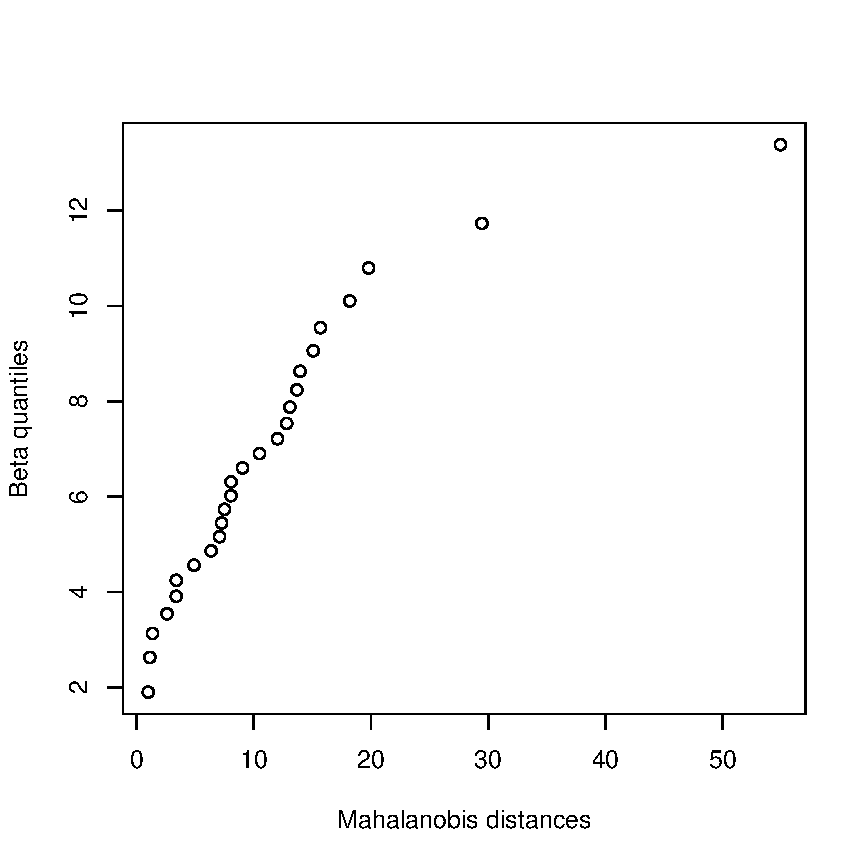
\includegraphics[width = 0.6\textwidth]{images/qqd1}
\caption{Mahalanobis distance from three component representation of the Heptathalon data versus theoretical quantiles of the Beta(1.5, 10) distribution}
\label{qqd1}
\end{center}
\end{figure}

It is reasonably clear from figure \ref{qqd1} that there are reasons to doubt multivariate normality, particularly in relation to outliers.    

Nevertheless, if we persevere, the adequacy of the $q=3$ dimensional representation can be considered.   Plotting $\delta_{a}^{2}$ against  $\delta_{b}^{2}$ provides one way of identifying those points not well represented by the three dimensional projection.

\singlespacing
\begin{verbatim}
> plot(hept.m$d1, hept.m$d2, 
  xlab = "Represented by q", ylab = "Not represented by q", 
  main = "Mahalanobis distances")
> identify(hept.m$d1, hept.m$d2, row.names(hept.df))
\end{verbatim}
\onehalfspacing

%It is equally possible to consider the mahalanobis distance in conventional desnsity plots.

%\singlespacing
%\begin{verbatim}
%library(MASS)
%truehist(hept.m$dtot, nbins = 9, ylim = c(0,0.1))
%curve(dchisq(x, df = 7), add = TRUE)
%\end{verbatim}
%\onehalfspacing

%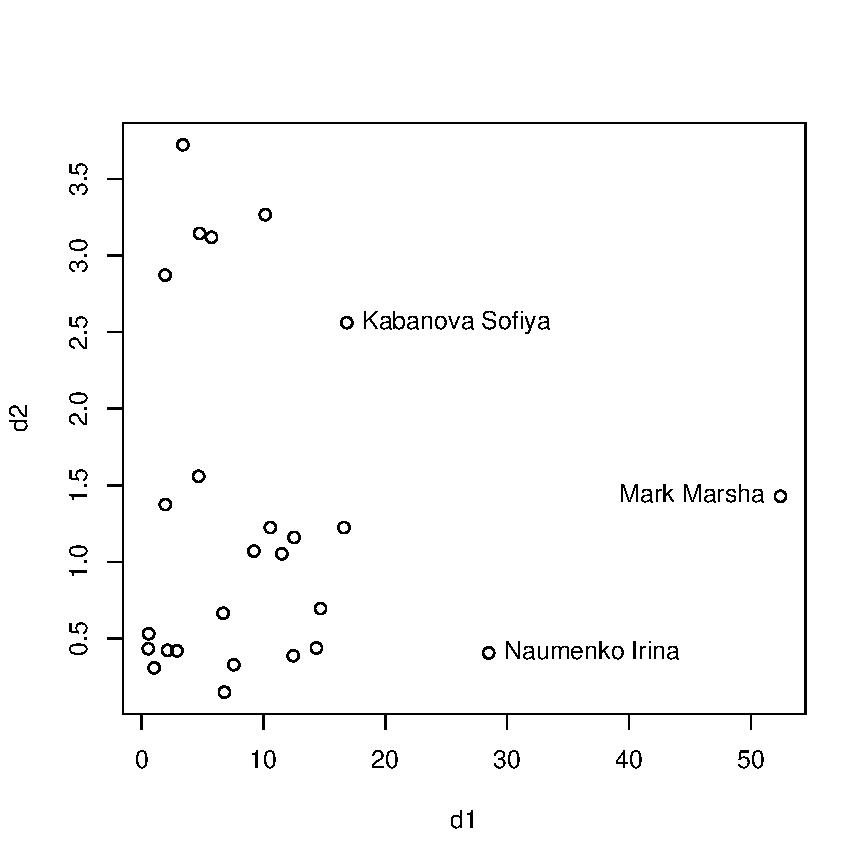
\includegraphics{images/d1d2}

%It should be noted that our ``outlier'' is only an outlier in the sense that she is not adequately represented by the first three principal components.   

However, qq plots of the data do tend to suggest that she could be considered an outlier.   This takes us back to the start of the chapter; in this case we may wish to consider a robust principal component analysis.

\singlespacing
\begin{verbatim}
> hep.princomp <- princomp(hept.df[-1], cor = TRUE)
> hep.cor.rob <- cov.rob(hept.df[,-1], cor = TRUE)$cor
> hep.princomp.rob <- princomp(cov = hep.cor.rob)
> hep.princomp
> hep.princomp.rob
> loadings(hep.princomp)
> loadings(hep.princomp.rob)
\end{verbatim}
\onehalfspacing

In this case it should be seen that there is only a slight difference between the estimates for the eigenvalues, but the loadings do alter somewhat.   Further methods for robust principal components will be considered in the next chapter.


\section{Interpreting the principal components}

This is the area that gets principal components a bad name.   Sometimes referred to as \textit{reification}, we look at the loadings on the various components, and try to suggest a concept that the component may be referring to.    Factor analysis does something similar.

It is worth at this point considering the correlation between a given variable and the principal component score (or projection of the data in $q$ dimensional subspace).

\begin{definition}
The univariate correlation between a variable and it's principal compnent projection can be given by:
\begin{displaymath}
\rho_{z,x_{k}} = \frac{e_{i}, \lambda_{i}}{\sqrt{\sigma_{kk}}}
\end{displaymath}
\end{definition}
\textbf{Proof}:[page 462] \cite{Johnson+Wichern:2002}

It should be noted that this only measures the unvariate contribution of $x$ to $z$, something \cite{Rencher:2002} feels is useless but something which may serve as a means to an end.

The corresponding measure for principal component analysis based on the correlation matrix is given by:
$\rho_{z, x_{standardised}} = e_{ik} \sqrt{\lambda_{i}}$


\section{Exercises}

\begin{enumerate}

\item Consider data $\boldsymbol{X} = \left( \begin{array}{ccc} 1 & 2 & 3 \\ 1 & 2 & 3 \end{array} \right) $.   Find the covariance and correlation matrix for these data.

\item Consider $\boldsymbol{S} = \left( \begin{array}{cc} 5 & 2 \\ 2 & 1 \end{array} \right) $.   Convert $\boldsymbol{S}$ into $\boldsymbol{R}$.   Calculate the principal components from each matrix.   Comare and contrast.   

\item Calculate $\rho_{z, x}$

\item S = diag(2,4,2), what are evals and evecs

\item Couple of questions on equicorrelation matrices

\item Estimate Sx and Sx.

\item Carapace data - how many pcs (sphericity test, bootstrap, scree, blah blah blah)

\end{enumerate}

%%% Local Variables: ***
%%% mode:latex ***
%%% TeX-master: "../book.tex"  ***
%%% End: ***
